% OBSERVAÇÃO: COMPILE PELO LUALATEX. CASO AINDA TENHA ALGUM CONFLITO NA COMPILAÇÂO FAÇA O SEGUINTE PROCEDIMENTO:
% COMPILE USANDO O XELATEX (ABA MENU -> SETTINGS -> COMPILLER -> XELATEX) E APÒS COMPILAR E GERAR O PDF, COMPILE NOVAMENTE SÓ QUE
% ALTERANDO O COMPILADOR PARA LUALATEX.
\documentclass[12pt, a4paper]{report} 
\usepackage{graphicx}
%\usepackage{xcolor}
\usepackage[table]{xcolor}
\usepackage[small]{caption}
%\usepackage[caption=false]{subfig}
\usepackage{subfigure}
\usepackage{float} % Para usar [H]
%\usepackage{bbm}
\usepackage{amsmath, amssymb}
\usepackage[T1]{fontenc}
%\usepackage[utf8]{inputenc}
%\usepackage[portuguese]{babel}
\usepackage[brazilian]{babel} %Indica a língua a ser escrita
\usepackage[normalem]{ulem}
%\usepackage[left=00cm, right=00cm, top=0.5cm, bottom=1.5cm]{geometry}
\usepackage{parskip}
\usepackage{color}
\usepackage{colortbl}
\usepackage{array}
\usepackage{setspace}
\usepackage{minted}
\usepackage{hyperref} 
\hypersetup{colorlinks=true, citecolor=blue, linkcolor=blue, urlcolor=blue}
	\usemintedstyle{perldoc}
\usepackage{multirow}
\usepackage{fancyhdr}
\usepackage{multicol}
\usepackage{balance} % Para equilibrar as colunas
\usepackage{indentfirst}
\usepackage{epstopdf}
\usepackage{animate}
\usepackage{xmpmulti}
\usepackage{multimedia}
\usepackage{wrapfig}
\usepackage{setspace}
\usepackage{pdfpages}
\usepackage{braket}

%------------------------------------------------------------------
% Cores - Sugestão: use uma cor parecida com a cor base (indico o site https://www.colorhexa.com/ para verificar os códigos de acordo com a cor da sua preferência)
\definecolor{base}{HTML}{3CA832} % Cor hexadecimal da edição (altere de acordo com a sua preferência)  EX: 893B4E
\definecolor{baseshadow}{HTML}{674DB2} % Cor hexadecimal do sombreamento dos textos na edição 
\definecolor{baseechoshadow}{HTML}{C4BAE1} % Cor hexadecimal do sombreamento do sombreamento dos textos na edição 
\setlength{\columnsep}{1cm}

%------------------------------------------------------------
% Comando para títulos de artigos
\usepackage{tikz}
\usetikzlibrary{calc} %Bibliotecas TikZ
\newcommand{\mytitle}[1]{%
    \newpage
    \phantomsection
    \begin{LARGE}
        \begin{center}
            \textcolor{base}{\textit{#1}}
        \end{center}
    \end{LARGE}
     \markboth{#1}{#1} % Define o marcador do cabeçalho
}
% Comando para subtítulos de títulos de artigos
\newcommand{\mytitlesubtitle}[1]{%
    \vspace{-.2cm}
    \begin{Large}
        \begin{center}
            \textcolor{base}{\textit{#1}}
        \end{center}
    \end{Large}
}
% Comando para subtítulos de artigos
\newcommand{\mysubtitle}[1]{%
       \phantomsection
       \vspace{5pt} % Espaço acima do subtítulo
       \begin{flushleft}
            \textcolor{base}{\textbf{#1}}
       \end{flushleft}
     \vspace{5pt} % Espaço abaixo do subtítulo
}

% Configurando o cabeçalho
\pagestyle{fancy}
\fancyhf{}

% Redefinindo a linha do cabeçalho com a cor e largura desejadas
\renewcommand{\headrule}{%
    \color{base} % Define a cor da linha
    \hrule width\headwidth height4pt % Define a largura da linha
    \vskip-\headrulewidth % Eleva a linha
}

% Garantir que a linha cubra toda a largura da página
\fancyheadoffset[L]{\dimexpr\hoffset+2cm\relax} % Alinhar à esquerda com a margem esquerda
\fancyheadoffset[R]{\dimexpr\hoffset+2cm\relax} % Alinhar à direita com a margem direita
\fancyhead[L]{\textcolor{base}
{\MakeUppercase{\large{\bf\hspace{0.3cm}\leftmark}}\vspace{0.35cm}}}
\setlength{\headheight}{33pt} % Ajuste o valor conforme necessário para consertar o erro headheight quando surgir
\setlength{\headsep}{35pt} % Ajusta a distância entre o cabeçalho e o texto
\fancyfoot[C]{\thepage} % Numeração das páginas
%\usepackage{flushend} % Pode ajudar a corrigir problemas de alinhamento
% Definindo um estilo sem cabeçalho, mas com numeração de página
\fancypagestyle{noheader}{
  \fancyhf{} % Limpa cabeçalhos e rodapés
  \renewcommand{\headrule}{%
    \color{base} % Define a cor da linha
    \hrule width\headwidth height0pt % Exlui a linha do cabeçalho
    \vskip-\headrulewidth % Eleva a linha
}
  \fancyfoot[C]{\thepage} % Mantém o rodapé com numeração de página
}


\usepackage{lipsum}
%\usepackage{indentfirst}
\usepackage{anysize} % Para personalizar a largura das margens
%\usepackage[margin=0.7874in]{geometry} % Define as margens
\marginsize{2cm}{2cm}{0.5cm}{2cm} % Ordem: Esquerda, direita, superior, inferior. Padrão ABNT - Esquerda: 3 cm. Superior: 0.5 cm. Direita: 2 cm. Inferior: 2 cm.
%\usepackage{geometry}
\usepackage{marginnote}
\setlength{\parindent}{20pt} %Indentação do parágrafo
\usepackage{subcaption}
\usepackage{subfigure}

%FONTES
\usepackage{anyfontsize} % Permite o uso de tamanhos de fonte arbitrários, independentemente dos tamanhos padrão
\usepackage{microtype} % Ajuste de espaçamento entre letras
\usepackage{fontspec} % Pacote para usar fontes TrueType e OpenType (só funciona compilando em LuaLaTex)
\usepackage{enumitem} % Pacote para personalizar listas
\usepackage{shadowtext} % Pacote para adicionar sombras ao texto
\usepackage{setspace} % Pacote para aumentar ou diminuir o espaço entre linhas
\usepackage{contour} % Para contornos em textos

% Definindo a largura do contorno (altere se precisar)
%\contourlength{2pt} % Largura do contorno


% Comandos personalizados para as fontes 
\newfontfamily{\hammersmithone}[Path = ./Fontes/]{HammersmithOne-Regular}
\newfontfamily{\bebasneue}[Path = ./Fontes/]{BebasNeue-Regular}
\newfontfamily{\bebasneuebold}[Path = ./Fontes/]{BebasNeue-Bold}
\newfontfamily{\cooperheavy}[Path = ./Fontes/]{CooperHewitt-Heavy}
\newfontfamily{\cooperbold}[Path = ./Fontes/]{CooperHewitt-Bold}
\newfontfamily{\cooperbook}[Path = ./Fontes/]{CooperHewitt-Book}
\newfontfamily{\norwester}[Path = ./Fontes/]{Norwester}
\newfontfamily{\abrilfatface}[Path = ./Fontes/]{AbrilFatface-Regular}
\newfontfamily{\leaguespartanbold}[Path = ./Fontes/]{LeagueSpartan-Bold}
\newfontfamily{\glacialbold}[Path = ./Fontes/]{Glacial-indifference-bold}
\newfontfamily{\glacialregular}[Path = ./Fontes/]{Glacial-indifference-regular}
\newfontfamily{\clearsansthin}[Path = ./Fontes/]{ClearSans-Thin}
\newfontfamily{\clearsansbold}[Path = ./Fontes/]{ClearSans-Bold}


% Definir um comando para usar fontes com tamanhos e cores personalizadas
\newcommand{\myfontsizeNewstonCapa}{\fontsize{120pt}{0pt}\selectfont\color{white}}
\newcommand{\myfontsizeNewstonFolhaRosto}{\fontsize{56pt}{0pt}\selectfont\color{base}}
\newcommand{\myfontsizeJornalCapa}{\fontsize{82pt}{0pt}\selectfont\color{white}}
\newcommand{\myfontsizeJornalFolhaRosto}{\fontsize{23pt}{0pt}\selectfont\color{base}}
\newcommand{\myfontsizeTemaCapaVerticalECC}{\fontsize{15pt}{0pt}\selectfont\color{white}}
\newcommand{\myfontsizeTema}{\fontsize{37pt}{0pt}\selectfont\color{white}}
\newcommand{\myfontsizeTitulosArtigosCapa}{\fontsize{25pt}{0pt}\selectfont\color{white}}
\newcommand{\myfontsizeTitulosArtigosCapaDois}{\fontsize{20pt}{0pt}\selectfont\color{white}}
\newcommand{\myfontsizeTituloTema}{\fontsize{73pt}{0pt}\selectfont\color{white}}
\newcommand{\myfontsizeTituloTemaEsm}{\fontsize{75pt}{0pt}\selectfont\color{base}}
\newcommand{\myfontsizeColecaoData}{\fontsize{11pt}{0pt}\selectfont\color{base}}
\newcommand{\myfontsizeColecaoTema}{\fontsize{19pt}{0pt}\selectfont\color{gray}}
\newcommand{\myfontsizeDivulgacaoCientifica}{\fontsize{45pt}{0pt}\selectfont\color{white}}
\newcommand{\myfontsizeSumario}{\fontsize{82pt}{0pt}\selectfont\color{base}}
\newcommand{\myfontsizeSumarioData}{\fontsize{27pt}{0pt}\selectfont\color{base}}
\newcommand{\myfontsizeNewstonSumarioECC}{\fontsize{40pt}{0pt}\selectfont\color{white}}
\newcommand{\myfontsizeJornalSumarioECC}{\fontsize{17pt}{0pt}\selectfont\color{white}}
\newcommand{\myfontsizeEdAntSite}{\fontsize{10pt}{0pt}\selectfont\color{white}}
\newcommand{\myfontsizeTextoCC}{\fontsize{16pt}{0pt}\selectfont\color{white}}
\newcommand{\myfontsizeUsuario}{\fontsize{12pt}{0pt}\selectfont\color{white}}
\newcommand{\myfontsizeSumarioTitulos}{\fontsize{16pt}{0pt}\selectfont}
\newcommand{\myfontsizeSumarioResumo}{\fontsize{12pt}{0pt}\selectfont}
\newcommand{\myfontsizeequipe}{\fontsize{42.6pt}{48pt}\selectfont}
\newcommand{\myfontsizecolabbebas}{\fontsize{27pt}{48pt}\selectfont}
\newcommand{\myfontsizeEdition}{\fontsize{21.3pt}{48pt}\selectfont}
\newcommand{\myfontsizeEditionFolhaRosto}{\fontsize{18pt}{0pt}\selectfont}
\newcommand{\myfontsizeColaboradores}{\fontsize{12.6pt}{48pt}\selectfont}

% Comando personalizado para texto com sombra
\newcommand{\shadowedText}[2][black]{%
    \begin{tikzpicture}[baseline=(T.base)]
        \node[inner sep=0pt, outer sep=0pt, text=#1] (S) at (0.06, -0.06) {#2}; % Ajuste (x, y) conforme necessário para mudar a posição da sombra em relação ao texto.
        \node[inner sep=0pt, outer sep=0pt, text=white] (T) at (0, 0) {#2};
    \end{tikzpicture}%
}

% Comando para texto com sombra e efeito eco
\newcommand{\echoShadowText}[3]{%
    \begin{tikzpicture}[baseline=(T.base)]
        % Sombra principal com deslocamento maior
        \node[inner sep=0pt, outer sep=0pt, text=#1, opacity=0.6] (S1) at (0.08, -0.08) {#3};
        % Sombra secundária com deslocamento menor
        \node[inner sep=0pt, outer sep=0pt, text=#2, opacity=0.6] (S2) at (0.04, -0.04) {#3};
        % Texto principal
        \node[inner sep=0pt, outer sep=0pt, text=white] (T) at (0, 0) {#3};
    \end{tikzpicture}%
}

%
\usepackage{titlesec}
\usepackage{titletoc}

% Define o estilo dos títulos do sumário
\titlecontents{chapter}
  [0em] % Margem esquerda
  {\glacialbold} % Fonte e estilo do título
  {\contentslabel{2em}} % Largura da etiqueta
  {} % Texto à esquerda do título
  {\hspace{0.1em}\titlerule*[0.4pc]{.}\hspace{-0.3em}\contentspage} % Linha de pontos até o número da página  
  [\vspace{0.4em}] % Espaço abaixo do título

% Definindo um novo comando \newauthor para o Sumário
\newcommand{\newauthor}[2]{\glacialbold{#1} \glacialregular{#2}}

% Comando personalizado para adicionar um capítulo ao sumário com título, imagem e resumo
\newcommand{\addchaptersummary}[4]{
  \phantomsection
  \addcontentsline{toc}{chapter}{\protect\myfontsizeSumarioTitulos\MakeUppercase{#1}}
  \addtocontents{toc}{
    \protect\begin{minipage}[t][.7cm][t]{4cm} % Alinhamento superior
      \protect\includegraphics[width=6em, height=6em]{#2}
    \protect\end{minipage}%
    \protect\begin{minipage}[t][.3cm][t]{9cm}% Definindo largura fixa para a minipage de texto com alinhamento superior
      \protect\vspace{-6em} % Ajuste fino para alinhar o resumo do texto com o topo da figura (altere de acordo com o topo da figura)
      \protect\myfontsizeSumarioResumo\glacialregular{#3}\\
      \protect\vfill % Espaço flexível que empurra o texto do autor para baixo
      \protect\vfill% Ajuste fino para alinhar o nome do autor do texto com a base da figura (altere de acordo com a base da figura)
      \newauthor{Autor(a):}{#4} 
      \protect\vspace{.2cm} % Ajuste fino para espaçamento entre figura e resumo e próximo artigo do sumário
    \protect\end{minipage}\vfill}
}

%[t]{7em}
% Remove o título "Sumário"
\pretocmd{\tableofcontents}{\renewcommand{\contentsname}{}}{}{\undefined}
% Redefinir o título da bibliografia
\usepackage{etoolbox}
\usepackage{adjustbox}
\usepackage{bookmark} % Ajuda na criação de links corretos
% Redefine a cor dos links no sumário
\AtBeginDocument{
    \pretocmd{\tableofcontents}{\hypersetup{linkcolor=black}}{}{}
    \apptocmd{\tableofcontents}{\hypersetup{linkcolor=blue}}{}{}
}

% Definindo o comando \authorinfo
\newcommand{\authorinfo}[2]{\vspace{1cm}\noindent%
    \textbf{\small{\textit{Escrito por: \href{#2}{#1}}}}
}
\usepackage{microtype}

% Redefine the numbering format for enumerate
\renewcommand{\theenumi}{[\arabic{enumi}]}
\renewcommand{\labelenumi}{\theenumi\ }
% Adjust the spacing between the number and the text
\setlist[enumerate,1]{left=0em, labelsep=.3em}
% Define a command to combine multiple references into one set of brackets
\newcommand{\refdois}[2]{%
  \textbf{[}\ref{#1}%
  \ifx&#2&\else
    \textbf{, }\ref{#2}%
  \fi
  \textbf{]}%
}

% Define a command to combine up to three references into one set of brackets
\newcommand{\reftres}[3]{%
  \textbf{[}%
  \ifx&#1&%
    \else \ref{#1}%
  \fi%
  \ifx&#2&%
    \else \ifx&#1&%
      \ref{#2}%
    \else
      \textbf{, }\ref{#2}%
    \fi%
  \fi%
  \ifx&#3&%
    \else \ifx&#1&\ifx&#2&%
      \ref{#3}%
    \else
      \textbf{, }\ref{#3}%
    \fi%
    \else
      \textbf{, }\ref{#3}%
    \fi%
  \fi%
  \textbf{]}%
}
















 % Novos pacotes, comandos, etc, adicione no arquivo Structure.tex

% Troque a cor da edição, tamanho, fontes de letra, etc no arquivo Structure.tex

% Comandos referentes a Edição (altere aqui que serão alterados automaticamente nos lugares em que são apresentados no pdf - ajuste apenas os valores de espaçamento e posicionamento na seção em que aparecem, caso seja necessário)
\newcommand{\NumeroEdicao}{8}
\newcommand{\ColecaoEdicao}{2025}
\newcommand{\DataEdicao}{Abril}

\begin{document}

    \protect\newpage
\thispagestyle{empty}
% OBS: Coloque sempre o que você quer deixar de fundo na página como primeiro comando

% Imagem de fundo - crie um arquivo separado em tamanho A4 (210x297mm) no formato pdf
\begin{tikzpicture}[remember picture,overlay]
    % Inclui a imagem em segundo plano
    \node[anchor=center,inner sep=0pt] at (current page.center) {
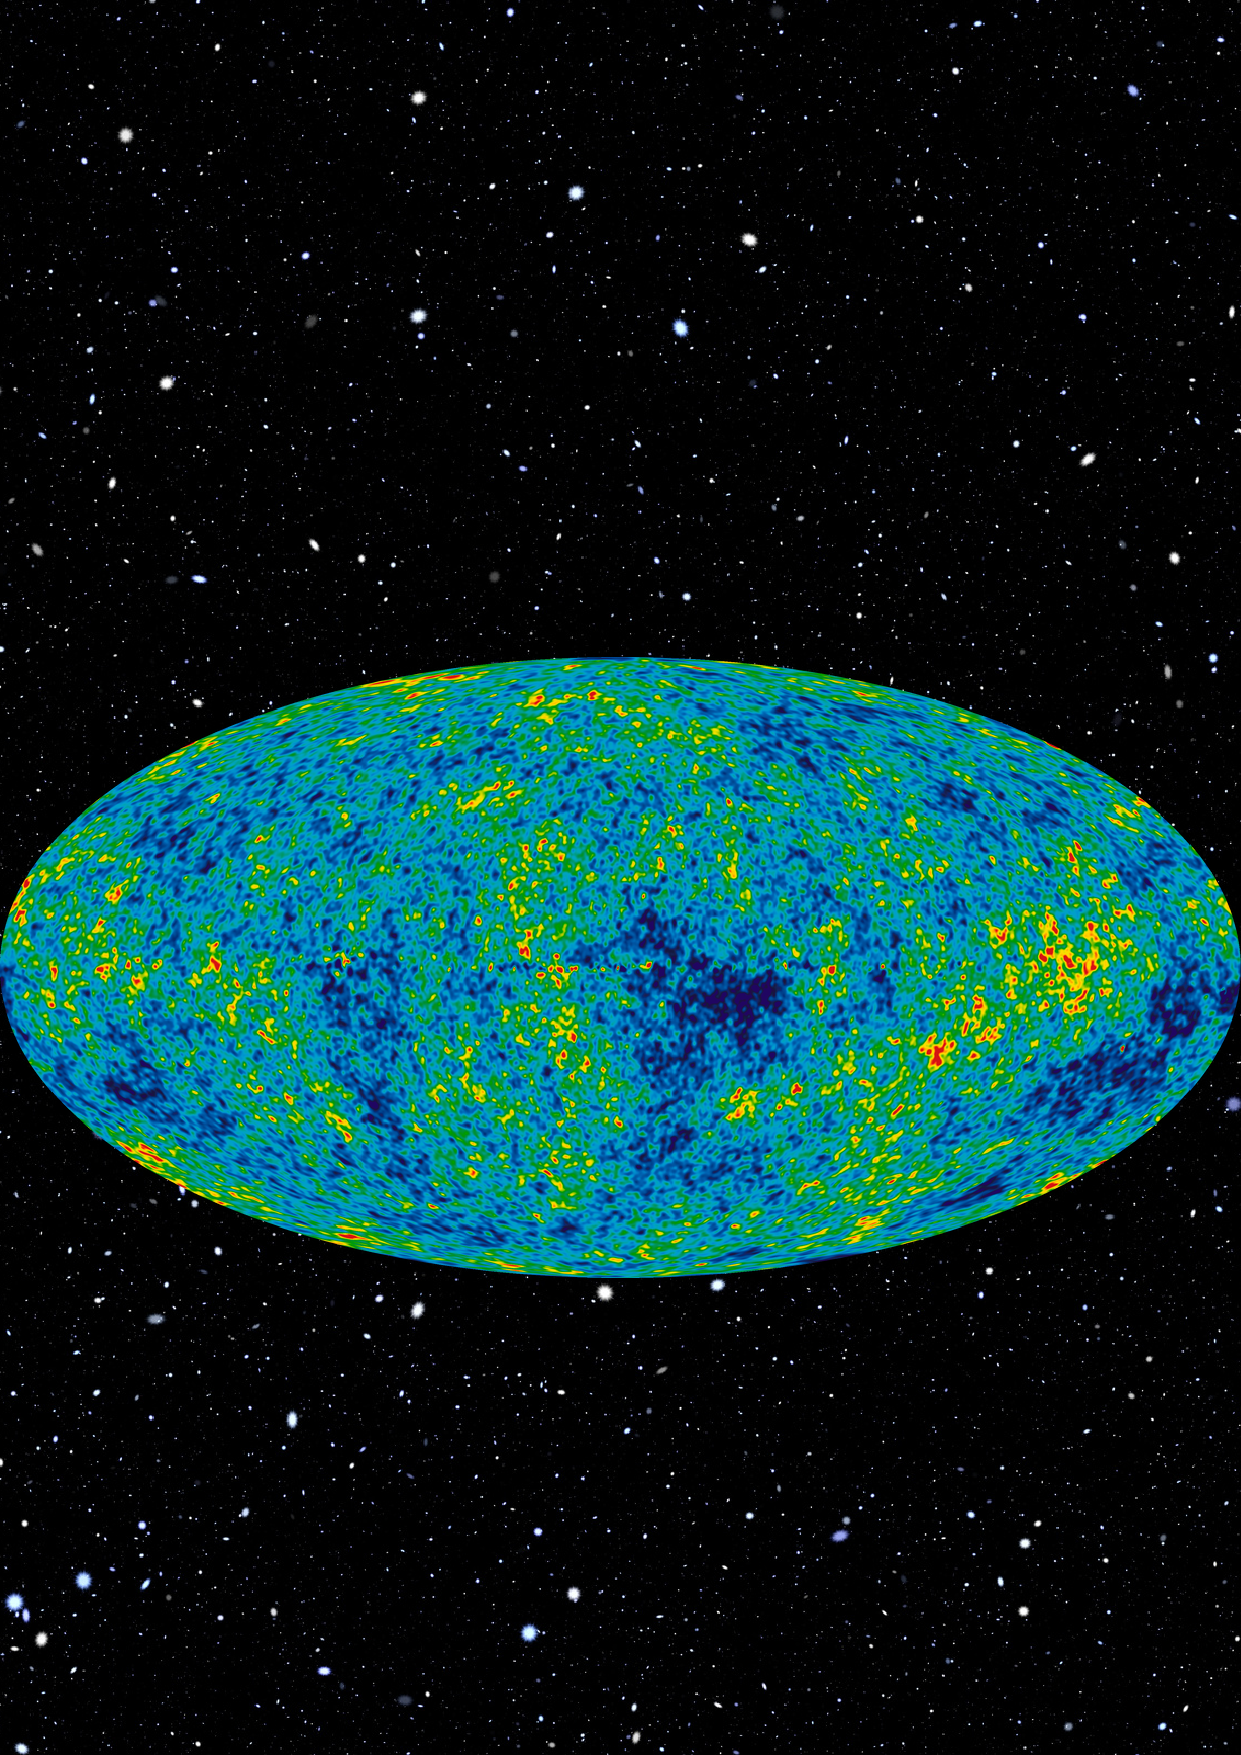
\includegraphics[width=\paperwidth,height=\paperheight,keepaspectratio]{Capa/Figuras_Capa/WMAP_Capa.pdf}
    };
\end{tikzpicture}

% Desenha um retângulo (branca)
\begin{tikzpicture}[remember picture, overlay]
    \draw[line width=7.4cm, white] 
        ($(current page.west) + (0,10.4)$) -- ($(current page.east) + (0,10.4)$);
\end{tikzpicture}

% Desenha um retângulo (cor da edição)
\begin{tikzpicture}[remember picture, overlay]
    \draw[line width=7cm, base] 
        ($(current page.west) + (0,10.4)$) -- ($(current page.east) + (0,10.4)$);
\end{tikzpicture}

% Nome da revista
\vspace{-3.2cm} % Ajuste a distância vertical para que o nome da revista fique centralizado com a linha horizontal
\begin{center}
    {\norwester\myfontsizeNewstonCapa NEWSTON}
\end{center}
\begin{center}
    {\bebasneue\myfontsizeJornalCapa \textls[530]{JORNAL}}
\end{center}

% Ajuste os valores em \textls[] (espaço entre letras) e na coordenada y de \node para adequar o tema e número com data da edição dentro do retângulo
\begin{tikzpicture}[remember picture, overlay]
    \node[anchor=north] at ($(current page.north west) + (0.5cm,-1.15cm)$) {
        \rotatebox{90}{\bebasneuebold\myfontsizeTemaCapaVerticalECC \textls[280]{HISTÒRIA\, DO\, UNIVERSO}}
    };
\end{tikzpicture}

\begin{tikzpicture}[remember picture, overlay]
    \node[anchor=north] at ($(current page.north west) + (20.5cm,-1.3cm)$) {
        \rotatebox{90}{{\bebasneuebold\myfontsizeTemaCapaVerticalECC \textls[200]{EDIÇÃO \NumeroEdicao -}} {\bebasneue\myfontsizeTemaCapaVerticalECC\textls[200]{\MakeUppercase{\DataEdicao}}}}
    };
\end{tikzpicture}

% Tema da edição
\hspace{-1.5cm}{\cooperheavy\myfontsizeTema\echoShadowText{baseechoshadow}{baseshadow}{História do Universo:}}

% Logo da UEM Branco
\begin{tikzpicture}[remember picture, overlay]
    % Ajuste a posição da figura conforme necessário
    \node[anchor=south, yshift=19cm, xshift=8cm] at (current page.south) { % Deslocamento vertical e horizontal na página - altere de acordo com o local em que deseja posicionar a logo
        
\includegraphics[width=0.23\textwidth]{Figuras_Capa_ContraCapa/UEM_Logo_Modelo_Branco.png}
    };
\end{tikzpicture}

% Desenha um retângulo (branca)
\begin{tikzpicture}[remember picture, overlay]
    \draw[line width=1.9cm, white] 
        ($(current page.west) + (0,-12.8)$) -- ($(current page.east) + (0,-12.8)$);
\end{tikzpicture}

% Desenha um retângulo (cor da edição) que engloba um título de artigo (diminua ou aumente a coordenada em x do segundo conjunto de coordenadas)
\begin{tikzpicture}[remember picture, overlay]
    \draw[line width=1.7cm, base] 
        ($(current page.west) + (0.1,-12.8)$) -- ($(current page.east) + (-12,-12.8)$);
\end{tikzpicture}

% Títulos de Artigos na Capa com TikZ (altere as coordenadas para posicionar o título do artigo dentro do retângulo de sua preferência)
\begin{tikzpicture}[remember picture, overlay]
    \node[anchor=north west, inner sep=0pt, outer sep=0pt] at ($(current page.north west) + (0.5cm,-27.2cm)$) {
        {\cooperbold\myfontsizeTitulosArtigosCapa Á Luz de Caravaggio}
    };
\end{tikzpicture}

% Desenha um retângulo (cor da edição) que engloba um título de artigo (diminua ou aumente a coordenada em x do primeiro e segundo conjunto de coordenadas)
\begin{tikzpicture}[remember picture, overlay]
    \draw[line width=1.7cm, base] 
        ($(current page.west) + (9.1,-12.8)$) -- ($(current page.east) + (-6.5,-12.8)$);
\end{tikzpicture}

% Títulos de Artigos na Capa com TikZ (altere as coordenadas para posicionar o título do artigo dentro do retângulo de sua preferência) para textos em duas linhas use \myfontsizeTitulosArtigosCapaDois para diminuir o tamanho da fonte
\begin{tikzpicture}[remember picture, overlay]
    \node[anchor=north west, inner sep=0pt, outer sep=0pt, text width=10cm] at ($(current page.north west) + (10cm,-27cm)$) {
        {\cooperbold\myfontsizeTitulosArtigosCapaDois Tipos de \\ Radiações}
    };
\end{tikzpicture}

\begin{tikzpicture}[remember picture, overlay]
    \draw[line width=1.7cm, base] 
        ($(current page.west) + (14.6,-12.8)$) -- ($(current page.east) + (-0.1,-12.8)$);
\end{tikzpicture}

\begin{tikzpicture}[remember picture, overlay]
    \node[anchor=north west, inner sep=0pt, outer sep=0pt, text width=10cm] at ($(current page.north west) + (15.5cm,-27cm)$) {
        {\cooperbold\myfontsizeTitulosArtigosCapaDois A Física dos\\ Esportes}
    };
\end{tikzpicture}


%{\cooperheavy\myfontsizeTituloTema ERA\\PRIMORDIAL}

%\begin{tikzpicture}[remember picture, overlay]
    %\node[anchor=center, inner sep=0pt, outer sep=0pt] at ([shift={(-1.5cm,-8.5cm)}] current page.center) {
      %  \begin{tikzpicture}
         % Múltiplos nós para criar um efeito de sombra esmaecida
        %    \foreach \angle in {0, 30, 60, 90, 120, 150, 180, 210, 240, 270, 300, 330} {
              %  \node[anchor=center, inner sep=0pt, outer sep=0pt, opacity=0.1, text=purple] at (\angle:0.2cm) {
               %     {\cooperheavy\myfontsizeTituloTema \shortstack[l]{ERA\\[0.5ex] PRIMORDIAL}}
              %  };
           % }
            % Texto principal
           % \node[anchor=center, inner sep=0pt, outer sep=0pt] {
             %   {\cooperheavy\myfontsizeTituloTema \shortstack[l]{ERA\\[0.5ex] PRIMORDIAL}}
          %  };
       % \end{tikzpicture}
  %  };
%\end{tikzpicture}

%\textcolor[gray]{\textopacity{0.5}{Este é um exemplo de texto esmaecido com opacidade de 50\%.}}


\begin{tikzpicture}[remember picture, overlay]
    \node[anchor=center, inner sep=0pt, outer sep=0pt] at ([shift={(-1.5cm,-8.5cm)}] current page.center) {
        \begin{tikzpicture}
             % Texto principal com contorno
            \node[anchor=center, inner sep=0pt, outer sep=0pt] {
                {\cooperheavy\myfontsizeTituloTema \contour{base}{\shortstack[l]{ERA\\[0.5ex] PRIMORDIAL}}}
            };
        \end{tikzpicture}
    };
\end{tikzpicture}



    \protect\newpage
\thispagestyle{empty}
% OBS: Coloque sempre o que você quer deixar de fundo na página como primeiro comando

% Imagem de fundo - crie um arquivo separado em tamanho A4 (210x297mm) no formato pdf
\begin{tikzpicture}[remember picture,overlay]
    % Inclui a imagem em segundo plano
    \node[anchor=center,inner sep=0pt] at (current page.center) {
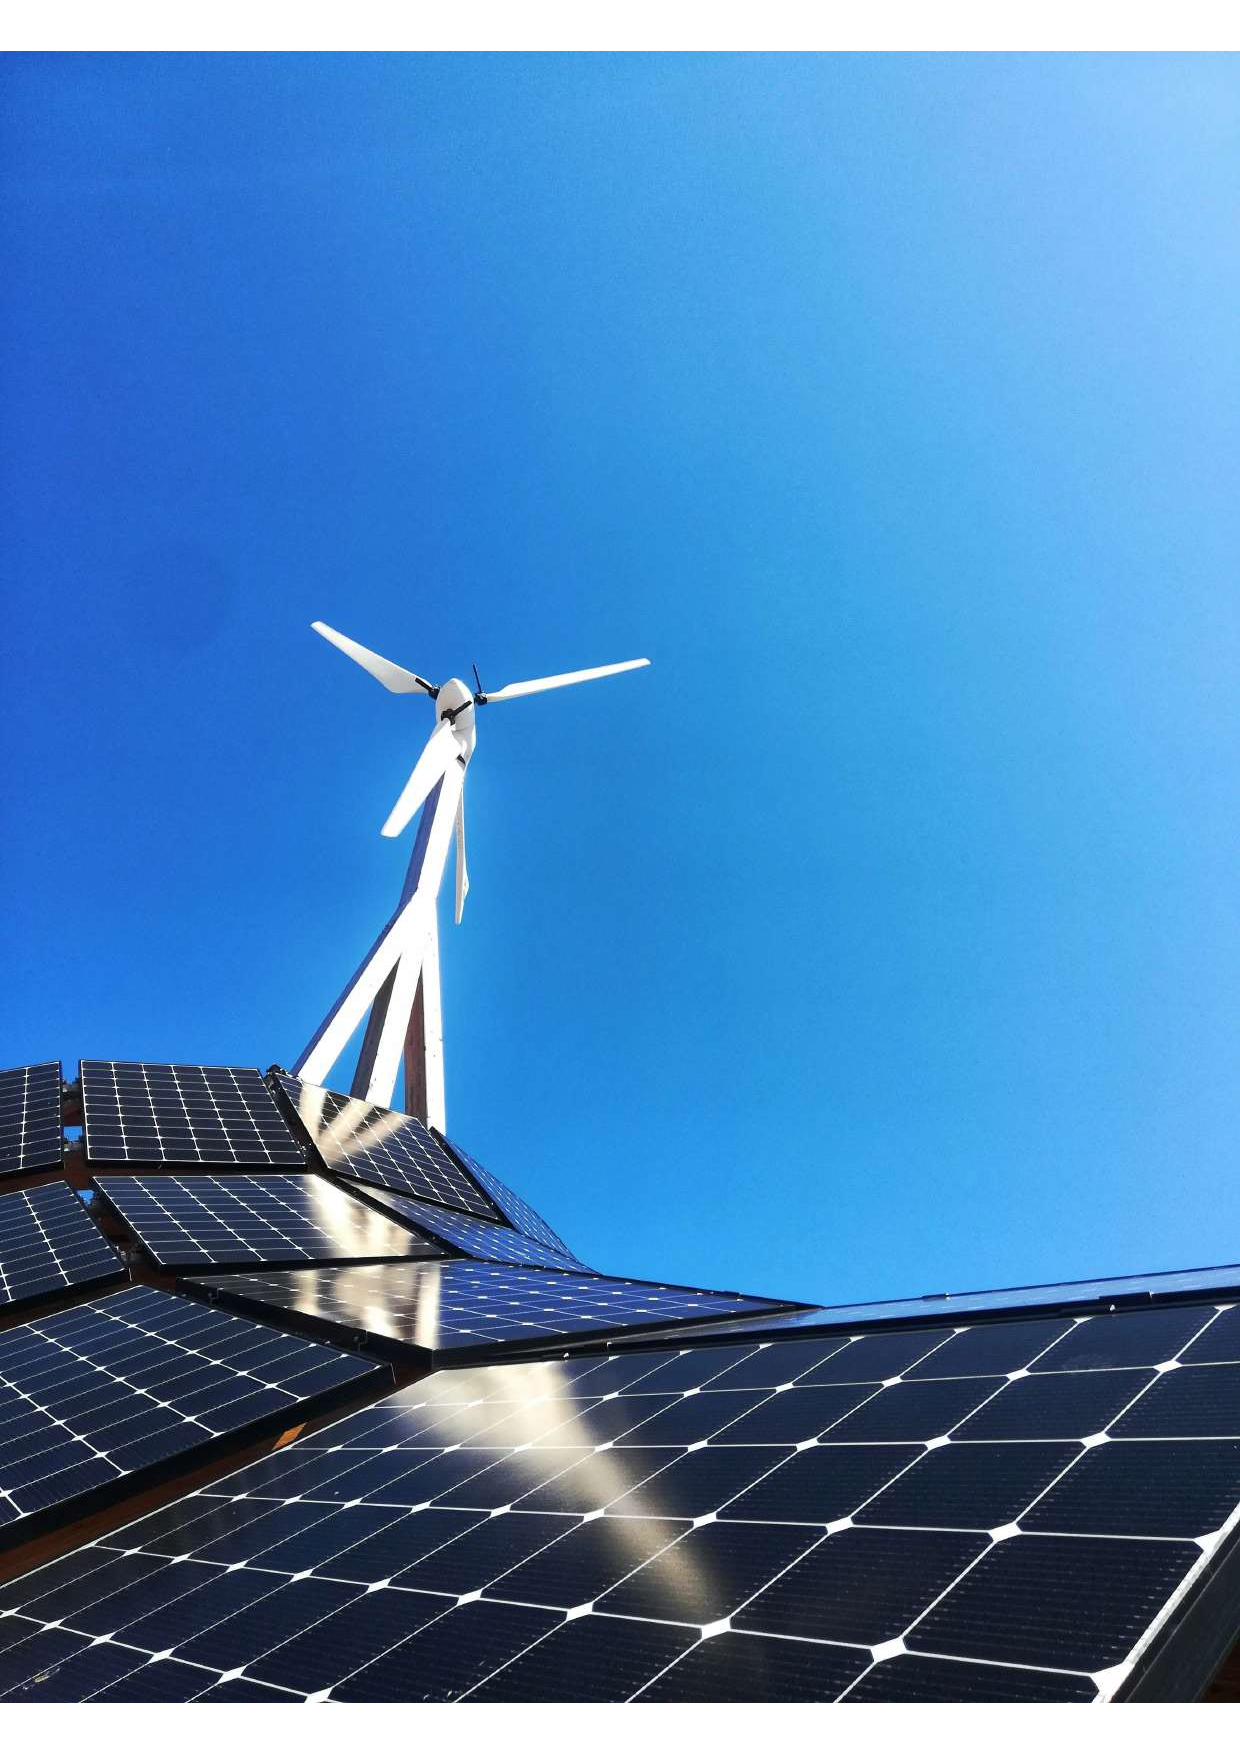
\includegraphics[width=\paperwidth,height=\paperheight,keepaspectratio]{Folha_Rosto/Figs_Folha_Rosto/solar-panel.pdf}
    };
\end{tikzpicture}

% Marcador de página branco
\begin{tikzpicture}[remember picture, overlay, x=1.1pt, y=1.1pt, yscale=-1, xscale=1]
    % Desenho do triângulo com altura aumentada
    \begin{scope}[yshift=-3cm, xshift=-7cm]
        \draw[fill=white, draw=white] 
            (181.51,363.13) -- (181.51,-192.01) -- (390.86,-192.01) -- 
            (390.86,363.13) -- (285.98,431.63) -- (181.56,363.13) -- 
            (181.51,363.13) -- cycle;
    \end{scope}
\end{tikzpicture}

%LOGO 
% Edite a imagem em um editor gráfico antes de incluí-la no documento LaTex. Ferramentas como GIMP, Inkscape, ou Photoshop podem ser usadas para alterar a cor da imagem (use o arquivo svg da pasta Figs_Folha_Rosto).
\begin{tikzpicture}[remember picture, overlay]
  % Adiciona a imagem com um deslocamento usando shift
  \node at (current page.north west) [anchor=north west, xshift=4.75cm, yshift=-0.9cm] {
    
\includegraphics[width=3.7cm]{Folha_Rosto/Figs_Folha_Rosto/divulga-logo.png}
  };
\end{tikzpicture}

% NOME DO JORNAL
% Altere a cor e/ou tamanho da fonte no comando \myfontsizeNewstonFolhaRosto e \myfontsizeJornalFolhaRosto  em Structure.tex caso queira outra que não seja a da edição
\begin{tikzpicture}[remember picture, overlay]
  % Adiciona o texto com um deslocamento usando shift
  \node at (current page.north west) [anchor=north west, xshift=4.48cm, yshift=-5.95cm] {
    {\norwester\myfontsizeNewstonFolhaRosto NEWSTON}
  };
   % Adiciona o texto com um deslocamento usando shift
  \node at (current page.north west) [anchor=north west, xshift=4.6cm, yshift=-7.1cm] {
    {\bebasneue\myfontsizeJornalFolhaRosto \textls[530]{JORNAL}}
  };
\end{tikzpicture}


%Número da Edição, coleção (se houver) e data (mês ano)
\begin{tikzpicture}[remember picture, overlay]
  % Desenhar a primeira linha
  \draw[line width=1mm, color=base, shift={(2, -1.5)}] (-1.3,-1) -- (5.4,-1);

  % Adicionar o círculo no meio da linha com um número dentro e preenchido com a cor base
  \node[circle, draw=base, fill=base, minimum size=1cm, inner sep=0pt, text=white, shift={(2, -1.5)}] at (2,-1) {\abrilfatface\myfontsizeEditionFolhaRosto \NumeroEdicao};

  % Adicionar a palavra "Coleção" entre as duas linhas
  \node[shift={(2, -2)}, anchor=center] at (0,-1) {\hammersmithone \myfontsizeColecaoData COLEÇÃO \ColecaoEdicao};

  % Adicionar outra palavra ao lado de "Coleção"
  \node[shift={(2, -2)}, anchor=center] at (4,-1) {\hammersmithone \myfontsizeColecaoData \MakeUppercase{\DataEdicao}};

  % Desenhar a segunda linha
  \draw[line width=1mm, color=base, shift={(2, -2.5)}] (-1.3,-1) -- (5.4,-1);

   % Desenhar uma linha pontilhada
   \foreach \i in {0.8, 0.95, 1.10, 1.25, 1.40, 1.55, 1.70, 1.85, 2, 2.15, 2.30, 2.45, 2.60, 2.75, 2.90, 3.05, 3.20} {
  \fill[base, shift={(0, -3.2)}] (\i+2, -1) circle (1pt);
};
  % Tema Principal
  \node[shift={(0, -5)}, anchor=center] at (4, -1) {
    \parbox{5cm}{\centering \hammersmithone \myfontsizeColecaoTema HISTÓRIA DO\\[1.5ex]UNIVERSO:\\[1.5ex]ERA PRIMORDIAL}
  };
  
  % Desenhar uma linha pontilhada
   \foreach \i in {0.8, 0.95, 1.10, 1.25, 1.40, 1.55, 1.70, 1.85, 2, 2.15, 2.30, 2.45, 2.60, 2.75, 2.90, 3.05, 3.20} {
  \fill[base, shift={(0, -6.9)}] (\i+2, -1) circle (1pt);
};
  % Logo UEM
   \node[shift={(0, -8.2)}, anchor=center] at (4, -1) {
\includegraphics[width=0.15\textwidth]{Figuras_Capa_ContraCapa/UEM_Logo_Modelo_Colorido.png}
    };
\end{tikzpicture}


\begin{tikzpicture}[remember picture, overlay]
  % Tema Principal
  \node[shift={(4.1, -15)}, anchor=center] at (5.7, -1) {
    \parbox{20cm}{\hammersmithone \myfontsizeDivulgacaoCientifica\textls[150]{DIVULGAÇÃO\\[0.4ex]CIENTÍFICA\\[1ex]E CULTURAL\\[1ex] PARA A\\[1ex]COMUNIDADE}}
  };
\end{tikzpicture}




    \protect\newpage
\thispagestyle{noheader}
% OBS: Coloque sempre o que você quer deixar de fundo na página como primeiro comando
% Adicione o TikZ para desenhar a linha vertical
\begin{tikzpicture}[remember picture, overlay]
    \draw[line width=10.8cm, black] ($(current page.north east) - (0,0)$) -- ($(current page.south east) - (0,0)$);
\end{tikzpicture}



\begin{tikzpicture}[remember picture, overlay]
  \node[shift={(0, 2.2)}, anchor=center] at (4,-1) {\leaguespartanbold\myfontsizeSumario Sumário};
  \node[shift={(-2.5, 0.2)}, anchor=center] at (4,-1) {\cooperbold \myfontsizeSumarioData \DataEdicao};
\end{tikzpicture}

% Adiciona um espaço vertical negativo para mover o sumário para cima
\vspace*{-0.2cm} % Ajuste este valor conforme necessário para que caibam mais itens de sumário numa mesma página

% Ajustar a largura do sumário usando adjustbox
\makebox[0pt][l]{
    \begin{adjustbox}{valign=t,minipage={.8\textwidth},margin={-3.5em,0pt}}
        {\myfontsizeSumarioTitulos\glacialbold
       \tableofcontents}
    \end{adjustbox}
}

%LOGO, NOME DO JORNAL e outras informações do canto direito da página de Sumário
%Edite a imagem em um editor gráfico antes de incluí-la no documento LaTex. Ferramentas como GIMP, Inkscape, ou Photoshop podem ser usadas para alterar a cor da imagem (use o arquivo svg da pasta Figs_Folha_Rosto).
% Altere a cor e/ou tamanho no comando \myfontsizeNewstonSumario \myfontsizeJornalSumarioECC em Structure.tex caso queira outra que não seja a da edição
\begin{tikzpicture}[remember picture, overlay]
  % Adiciona a logo maçã branco
%  \node at (current page.north west) [anchor=north west, xshift=16.8cm, yshift=-0.7cm] {
%    
\includegraphics[width=2.5cm]{Sumario/Figs_Sumario/Logo_Maca_Branco.png}
%  };
    % Adiciona o texto Newston
  \node at (current page.north west) [anchor=north west, xshift=15.8cm, yshift=-1cm] {
    {\norwester\myfontsizeNewstonSumarioECC DIVULGA}
  };
   % Adiciona o texto Jornal
  \node at (current page.north west) [anchor=north west, xshift=15.9cm, yshift=-2.2cm] {
    {\bebasneue\myfontsizeJornalSumarioECC \textls[490]{AUTOMAÇÃO}}
  };
   % Adiciona o texto Edições Anteriores
  \node at (current page.north west) [anchor=north west, xshift=16.25cm, yshift=-7.5cm] {
    \parbox{20cm}{\glacialbold\myfontsizeEdAntSite ACESSE AS EDIÇÕES \\[0.4ex] ANTERIORES}
  };
  % Ícone site
   \node at (current page.north west) [anchor=north west, xshift=16.2cm, yshift=-8.5cm] {
    
\includegraphics[width=.5cm]{Sumario/Figs_Sumario/Icone_Site.png}
  };
  % Site
  \node at (current page.north west) [anchor=north west, xshift=16.8cm, yshift=-8.55cm] {
    {\glacialregular\myfontsizeEdAntSite \href{https://posautomacao.ufsc.br/revista-ppgeas/}{\textls[50]{posautomacao.ufsc.br}}}
  };
   % Adiciona o texto Fale Conosco...
  \node at (current page.north west) [anchor=north west, xshift=16.25cm, yshift=-20.5cm] {
    \parbox{20cm}{\glacialbold\myfontsizeEdAntSite FALE CONOSCO POR \\[0.8ex] NOSSAS REDES \\[0.8ex] SOCIAIS}
  };
%  % Ícone Insta
%   \node at (current page.north west) [anchor=north west, xshift=16.25cm, yshift=-21.8cm] {
%    
\includegraphics[width=.6cm]{Sumario/Figs_Sumario/Icone_Insta.png}
%  };
%  % Ícone Face
%   \node at (current page.north west) [anchor=north west, xshift=17.25cm, yshift=-21.8cm] {
%    
\includegraphics[width=.6cm]{Sumario/Figs_Sumario/Icone_Facebook.png}
%  };
%  % Ícone X
%   \node at (current page.north west) [anchor=north west, xshift=18.25cm, yshift=-21.8cm] {
%    
\includegraphics[width=.6cm]{Sumario/Figs_Sumario/Icone_X.png}
%  };
  % Usuario
  \node at (current page.north west) [anchor=north west, xshift=16.25cm, yshift=-22cm] {
    {\bebasneue\myfontsizeUsuario \textls[150]{@DIVULGAAUTOMACAO}}
  };
%  % Ícone e-mail
%   \node at (current page.north west) [anchor=north west, xshift=16.25cm, yshift=-23.25cm] {
%    
\includegraphics[width=.5cm]{Sumario/Figs_Sumario/Icone_Email.png}
%  };
  % e-mail
%  \node at (current page.north west) [anchor=north west, xshift=16.9cm, yshift=-23.33cm] {
%    {\glacialregular\myfontsizeEdAntSite \textls[50]{newston@uem.br}}
%  };
  % Adiciona a logo da UEM branco
  \node at (current page.north west) [anchor=north west, xshift=16.4cm, yshift=-24.7cm] {
    
\includegraphics[width=3.7cm]{Figuras_Capa_ContraCapa/ufsc-bw.png}
  };
\end{tikzpicture}





    \protect\newpage
\thispagestyle{noheader}
% Adicione o TikZ para desenhar a linha vertical
\begin{tikzpicture}[remember picture, overlay]
    \draw[line width=3.4cm, base] ($(current page.north east) - (0,0)$) -- ($(current page.south east) - (0,0)$);
\end{tikzpicture}

\noindent{\hammersmithone\myfontsizeequipe\textls[155]{EQUIPE}}

\vspace{0.3cm} 

\noindent\hspace{0.1cm}{\bebasneue\myfontsizecolabbebas
\textls[235]{COLABORADORES\, DO\, JORNAL}
}

\vspace{0.3cm} 
% Número da Edição
\noindent\hspace{0.1cm}{\cooperbold\myfontsizeEdition
\textls[100]{Newston Jornal - Ed. \NumeroEdicao}
}

\vspace{0.3cm} 
% Mês e ano da Edição
\noindent\hspace{0.1cm}{\cooperbook\myfontsizeEdition
\textls[100]{\DataEdicao}
}

\vspace{1cm}

% Para adicionar novo colaborador copie e cole o ambiente a seguir logo abaixo e faça as devidas alterações. Na parte do e-mail mantenha "mailto:" antes do e-mail para que ao clicar sobre o e-mail no PDF o leitor seja direcionado para sua caixa de e-mail padrão

\begin{itemize}
    \item {\cooperbold\myfontsizeColaboradores \textls[100]{Breno Ferraz de Oliveira}} % Nome
    {\cooperbook\myfontsizeColaboradores \textls[100]{(\href{mailto:breno@dfi.uem.br}{breno@dfi.uem.br})}} % E-mail
    \begin{itemize}[label={\raisebox{0.4ex}{\color{black}\scalebox{0.3}{\textcircled{\color{white}\textbullet}}}}, labelsep=0.5em] % Define o símbolo como um círculo branco com contorno preto
        \item {\cooperbook\myfontsizeColaboradores \textls[100]{Orientador - Professor DFI/UEM}}% Cargo na revista - Formação acadêmica e/ou Departamento/Universidade 
    \end{itemize}
\end{itemize}

\begin{itemize}
    \item {\cooperbold\myfontsizeColaboradores \textls[100]{Fernando Carlos Messias Freire}} % Nome
    {\cooperbook\myfontsizeColaboradores \textls[100]{(\href{mailto:fcmfreire@uem.br}{fcmfreire@uem.br})}} % E-mail
    \begin{itemize}[label={\raisebox{0.4ex}{\color{black}\scalebox{0.3}{\textcircled{\color{white}\textbullet}}}}, labelsep=0.5em] % Define o símbolo como um círculo branco com contorno preto
        \item {\cooperbook\myfontsizeColaboradores \textls[100]{Orientador - Professor DFI/UEM}}% Cargo na revista - Formação acadêmica e/ou Departamento/Universidade 
    \end{itemize}
\end{itemize}

\begin{itemize}
    \item {\cooperbold\myfontsizeColaboradores \textls[100]{Alexandre Alabora}} % Nome
    {\cooperbook\myfontsizeColaboradores \textls[100]{(\href{mailto:alexandre.alabora@gmail.com}{alexandre.alabora@gmail.com})}} % E-mail
    \begin{itemize}[label={\raisebox{0.4ex}{\color{black}\scalebox{0.3}{\textcircled{\color{white}\textbullet}}}}, labelsep=0.5em] % Define o símbolo como um círculo branco com contorno preto
        \item {\cooperbook\myfontsizeColaboradores \textls[100]{Editor - Bacharel em Física/UEM}}% Cargo na revista - Formação acadêmica e/ou Departamento/Universidade 
    \end{itemize}
\end{itemize}

\begin{itemize}
    \item {\cooperbold\myfontsizeColaboradores \textls[100]{Vítor Hugo Ribeiro}} % Nome
    {\cooperbook\myfontsizeColaboradores \textls[100]{(\href{mailto:vitorhibeiro@gmail.com}{vitorhibeiro@gmail.com})}} % E-mail
    \begin{itemize}[label={\raisebox{0.4ex}{\color{black}\scalebox{0.3}{\textcircled{\color{white}\textbullet}}}}, labelsep=0.5em] % Define o símbolo como um círculo branco com contorno preto
        \item {\cooperbook\myfontsizeColaboradores \textls[100]{Editor e Design da Edição - Mestrando em Física/UNICAMP}}% Cargo na revista - Formação acadêmica e/ou Departamento/Universidade 
    \end{itemize}
\end{itemize}

\begin{itemize}
    \item {\cooperbold\myfontsizeColaboradores \textls[100]{Luiz Felipe Demétrio}} % Nome
    {\cooperbook\myfontsizeColaboradores \textls[100]{(\href{mailto:demetrio.luizfelipe.fis@gmail.com}{demetrio.luizfelipe.fis@gmail.com})}} % E-mail
    \begin{itemize}[label={\raisebox{0.4ex}{\color{black}\scalebox{0.3}{\textcircled{\color{white}\textbullet}}}}, labelsep=0.5em] % Define o símbolo como um círculo branco com contorno preto
        \item {\cooperbook\myfontsizeColaboradores \textls[100]{Redator/Revisor - Mestrando em Física/UEL}}% Cargo na revista - Formação acadêmica e/ou Departamento/Universidade 
    \end{itemize}
\end{itemize}

\begin{itemize}
    \item {\cooperbold\myfontsizeColaboradores \textls[100]{Milena Camila Fernandes}} % Nome
    {\cooperbook\myfontsizeColaboradores \textls[100]{(\href{mailto:milenaffernandes@outlook.com}{milenaffernandes@outlook.com})}} % E-mail
    \begin{itemize}[label={\raisebox{0.4ex}{\color{black}\scalebox{0.3}{\textcircled{\color{white}\textbullet}}}}, labelsep=0.5em] % Define o símbolo como um círculo branco com contorno preto
        \item {\cooperbook\myfontsizeColaboradores \textls[100]{Redatora - Mestra em Física/UEM}}% Cargo na revista - Formação acadêmica e/ou Departamento/Universidade 
    \end{itemize}
\end{itemize}

\begin{itemize}
    \item {\cooperbold\myfontsizeColaboradores \textls[100]{Murilo Aparecido da Silva}} % Nome
    {\cooperbook\myfontsizeColaboradores \textls[100]{(\href{mailto:muriloas.work@gmail.com}{muriloas.work@gmail.com})}} % E-mail
    \begin{itemize}[label={\raisebox{0.4ex}{\color{black}\scalebox{0.3}{\textcircled{\color{white}\textbullet}}}}, labelsep=0.5em] % Define o símbolo como um círculo branco com contorno preto
        \item {\cooperbook\myfontsizeColaboradores \textls[100]{Redator - Mestrando em Física/UEM}}% Cargo na revista - Formação acadêmica e/ou Departamento/Universidade 
    \end{itemize}
\end{itemize}

\begin{itemize}
    \item {\cooperbold\myfontsizeColaboradores \textls[100]{Milena Chierrito}} % Nome
    {\cooperbook\myfontsizeColaboradores \textls[100]{(\href{mailto:milenachierrito@gmail.com}{milenachierrito@gmail.com})}} % E-mail
    \begin{itemize}[label={\raisebox{0.4ex}{\color{black}\scalebox{0.3}{\textcircled{\color{white}\textbullet}}}}, labelsep=0.5em] % Define o símbolo como um círculo branco com contorno preto
        \item {\cooperbook\myfontsizeColaboradores \textls[100]{Revisora - Arquitetura e Urbanismo/UEM}}% Cargo na revista - Formação acadêmica e/ou Departamento/Universidade 
    \end{itemize}
\end{itemize}

\begin{itemize}
    \item {\cooperbold\myfontsizeColaboradores \textls[100]{Sanderson Carlos Ribeiro}} % Nome
    {\cooperbook\myfontsizeColaboradores \textls[100]{(\href{mailto:San.Car.Oficial@gmail.com}{San.Car.Oficial@gmail.com})}} % E-mail
    \begin{itemize}[label={\raisebox{0.4ex}{\color{black}\scalebox{0.3}{\textcircled{\color{white}\textbullet}}}}, labelsep=0.5em] % Define o símbolo como um círculo branco com contorno preto
        \item {\cooperbook\myfontsizeColaboradores \textls[100]{Cartunista - Mestrando em Física/UEL}}% Cargo na revista - Formação acadêmica e/ou Departamento/Universidade 
    \end{itemize}
\end{itemize}

\begin{itemize}
    \item {\cooperbold\myfontsizeColaboradores \textls[100]{Andrey Karvat}} % Nome
    {\cooperbook\myfontsizeColaboradores \textls[100]{(\href{mailto:andrey.karvat123@hotmail.com}{andrey.karvat123@hotmail.com})}} % E-mail
    \begin{itemize}[label={\raisebox{0.4ex}{\color{black}\scalebox{0.3}{\textcircled{\color{white}\textbullet}}}}, labelsep=0.5em] % Define o símbolo como um círculo branco com contorno preto
        \item {\cooperbook\myfontsizeColaboradores \textls[100]{Webdesign - Física/UEM}}% Cargo na revista - Formação acadêmica e/ou Departamento/Universidade 
    \end{itemize}
\end{itemize}





    \protect% PAGINA INICIAL DO PRIMEIRO ARTIGO
\mytitle{A História do Universo: Era Primordial} % Título do Artigo    
\addchaptersummary{A História do Universo: Era Primordial}{Sumario/Figs_Sumario/FigArtigo1.jpg}{Neste texto aprenderemos sobre a origem dos átomos e também sobre a luz mais antiga do universo: a radiação cósmica de fundo, de 13,8 bilhões de anos.}{Luiz Felipe Demétrio} 
% Comando para adicionar o título do artigo (deve sempre ficar após o comando \mytitle) no sumário bem como uma figura, resumo e autor(a) do mesmo (obs: o diretório da figura deve ser especificado na segunda variável como mostra esse exemplo. Recomenda-se o uso de figuras quadradas.)
\newcommand{\artigoum}{\begin{center}\textcolor{base}{\MakeUppercase{A História do Universo: Era Primordial}}\end{center}} % Comando para adicionar o nome do artigo nas referências. Altere \artigoum para \artigodois, \artigotres de acordo com o total de artigos da edição e adicione o mesmo comando antes da sua seção no arquivo Referencias.tex

% Use o ambiente multicols para textos em duas colunas.
\begin{multicols}{2} % Tudo o que estiver dentro desse ambiente ficará no layout de duas colunas. 
% Pule uma linha entre \begin{multicols} e o texto
Bem-vindo a mais um texto sobre a História do Universo. Vimos no \href{https://drive.google.com/file/d/1D3q3ixp0qqPirSmoWL_jqtcO3WCsY0qJ/view}{último texto} que a fusão estelar não explica a origem dos elementos químicos leves, como hidrogênio e hélio. Mas, na verdade, eu enganei vocês: o buraco é bem mais embaixo. Veja bem, todos os elementos químicos são feitos de átomos. Mas de onde vem os átomos? Continue lendo e você descobrirá .

\mysubtitle{Rebobinando o filme do Universo} % Subtítulo do Artigo  
%

Como já vimos, o universo expande, e isso nos fornece muita informação sobre seu comportamento. Isso significa que, se ``rebobinarmos o filme'' do universo, então, no passado, ele deveria ter sido ``menor''\footnote{Lembrando que o universo é \textbf{infinito}, mas as \textbf{distâncias} dentro dele variam com o tempo.}, e, consequentemente, mais quente e denso\footnote{É isso que chamamos de \textit{Big Bang}: a ideia de que o universo evoluiu de um estado quente e denso para o que vemos hoje, capaz até de gerar vida.}.

% Para aspas duplas de abertura, use dois caracteres de acento grave (ou crase. Para aspas duplas de fechamento, use dois caracteres de aspas simples. Ex: ``palavra ou frase''. Use o comando \footnote{} para notas de rodapé.

Como as escalas de distância do universo primordial eram menores, isso se aplica também para os comprimentos de onda $\lambda$ da luz. A energia $E$ da luz em função de seu comprimento de onda é dada pela relação de Planck

\begin{equation}\label{Eq1}
    E = \frac{hc}{\lambda}\, ,
\end{equation}

\noindent em que $h$ é a constante de Planck e $c$ a velocidade da luz. Vemos então que energia e comprimento de onda são inversamente proporcionais: quanto menor o comprimento de onda, maior a energia. 

% Use o comando \noindent para tirar a indentação de um parágrafo e o comando \ref{} para citar a equação no texto de acordo com o seu rótulo no comando \label{Eq1}. 

Sabemos também que, no passado, o comprimento de onda da luz era menor, ou seja, ela possuía muito mais energia do que tem hoje em dia. Em particular, nas eras primordiais do universo, ela tinha energia suficiente para destruir átomos.

Uma forma de entender isso é imaginar um grupo de amigos abraçados em uma praia, como os da Figura \ref{fig:amigos}. Imagine agora que uma onda passa pelo nosso grupo de amigos, uma onda bem fraquinha. Como ela é fraca, ela irá apenas incomodar os amigos um pouco, mas não irá desfazer o abraço coletivo.

\begin{figure}[H]
	\centering
	
\includegraphics[width=\linewidth]{Figuras/Artigo1/Beach.png}
	\caption{Amigos de mãos dadas. Feito pelo autor no \href{https://www.canva.com/}{Canva}.}
	\label{fig:amigos}
\end{figure}

Porém, se a energia da onda aumentar, ela poderá vir a desfazer a roda, a não ser que os amigos façam mais força para se segurarem. Obviamente, se a onda for muito muito forte, eles jamais conseguirão manter o abraço coletivo.

Agora que entendemos nossa experiência imaginária na praia, voltemos para o universo primordial. A situação é totalmente análoga: os prótons e elétrons são muito amigos, e sentem uma atração (elétrica) muito forte, querendo ficar abraçados. O nome desses abraços coletivos são \textit{átomos} (Figura \ref{fig:bohr}). Na analogia, a onda faz o papel da luz.

\begin{figure}[H]
	\centering
	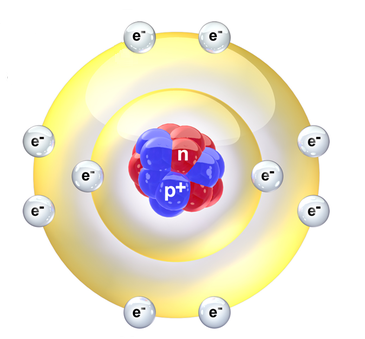
\includegraphics[width=0.9\linewidth]{Figuras/Artigo1/Bohr.png}
	\caption{Um átomo é composto por elétrons de cargas negativa, com um nucleon de prótons com carga positiva e nêutrons sem carga. Fonte: \href{https://en.wikipedia.org/wiki/File:Blausen_0342_ElectronEnergyLevels.png}{Wikipédia}.}
	\label{fig:bohr}
\end{figure}

\mysubtitle{Nucleossíntese primordial}

O universo primordial era então como uma praia cheia de ondas muito poderosas, que destruíam os átomos. Porém, conforme ele se expandiu, chegou a um ponto no qual as ondas foram perdendo energia, até que elas permitissem a formação de núcleos de átomos. Esse instante é muito importante para a História do Universo, sendo chamado de \textbf{Nucleossíntese Primordial}, e ocorreu cerca de 10 a 20 minutos depois do que chamamos de ``origem'' do universo.
	
Em seguida, ocorreu a chamada \textbf{Recombinação}, quando os núcleos capturaram elétrons e foram formados os primeiros átomos de hidrogênio, hélio, e outros elementos leves. Isso  ocorreu há cerca de 13,8 bilhões de anos, aproximadamente 380 mil anos depois da Nucleossíntese Primordial. Em seguida, conforme o universo evoluiu, eles se condensaram em elementos mais pesados, depois estrelas e galáxias.

A origem dos átomos por si só já é uma consequência incrível do modelo do Big Bang, pois a abundância de hidrogênio e hélio em nosso universo não é explicada por outros modelos cosmológicos.  Porém, surge uma outra pergunta: agora que a luz primordial perdeu energia e parou de colidir com os átomos e destruí-los, o que aconteceu com ela?

\mysubtitle{Radiação Cósmica de Fundo(CMB)}

Desde o momento da recombinação, os fótons\footnote{Partículas de luz.}  não conseguiram mais destruir os átomos, passando a vagar livremente pelo universo. Eles então vagaram e vagaram, por todo o cosmos, ou melhor, até a parte do cosmos que tiveram tempo de andar\footnote{Porque a velocidade da luz é finita.}. 

\begin{figure}[H]
	\centering
	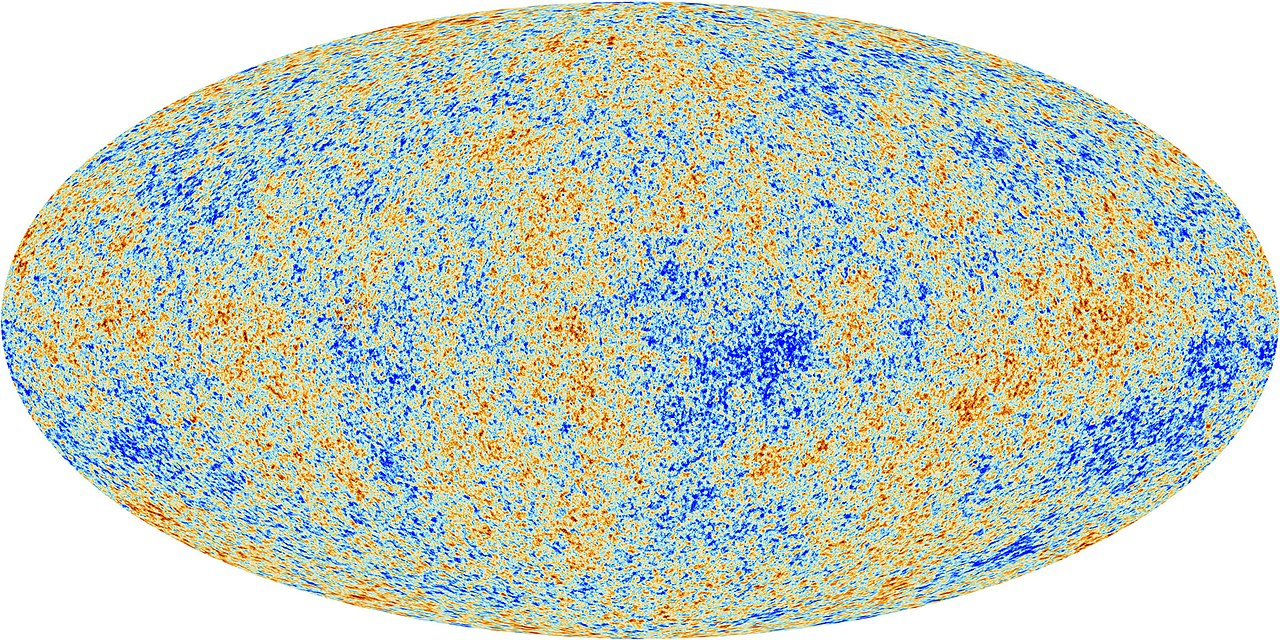
\includegraphics[width=0.9\linewidth]{Figuras/Artigo1/CMB.jpg}
	\caption{\small Mapa de calor da radiação cósmica de fundo (CMB). As regiões mais alaranjadas tem maior temperatura, enquanto as azuladas são mais frias. Fonte: \href{https://en.wikipedia.org/wiki/Cosmic_microwave_background}{Wikipédia}.}
	\label{fig:CMB}
\end{figure}

Mas o que diabos aconteceu com esses fótons vagantes, se nada mais havia para pará-los? A resposta é que eles andaram até onde conseguiram, e vários deles chegaram até a Terra. Sim, fótons/luz de 13,8 bilhões de anos chegaram até nós! Na verdade, a afirmação é mais forte ainda: luz de 13,8 bilhões de anos chegou até aqui na Terra, e está colidindo com você neste exato momento. Você está a todo momento sendo banhando de luz primordial!

Obviamente, quando fazemos afirmações fortes como ``luz primordial chegou até nós'', elas recebem um ar meio misterioso e até místico. Mas devo relembrá-lo de que este é um conceito científico: esta luz primordial já foi observada, e é essencial para a cosmologia moderna.

Chamamos essa luz, a mais antiga já vista pelo homem, de \textit{radiação cósmica de fundo} (CMB\footnote{Do inglês \textit{Cosmic Microwave Background Radiation}.}). Ela foi medida pela primeira vez por Penzias e Wilson em 1964 \ref{ref1:artigo1}.Na verdade, eles tentaram medir outro efeito, mas detectaram um sinal luminoso muito fraco, inicialmente atribuindo-o a falhas do equipamento. Na verdade, estavam descobrindo algo de muito profundo.

\begin{figure}[H]
	\centering
	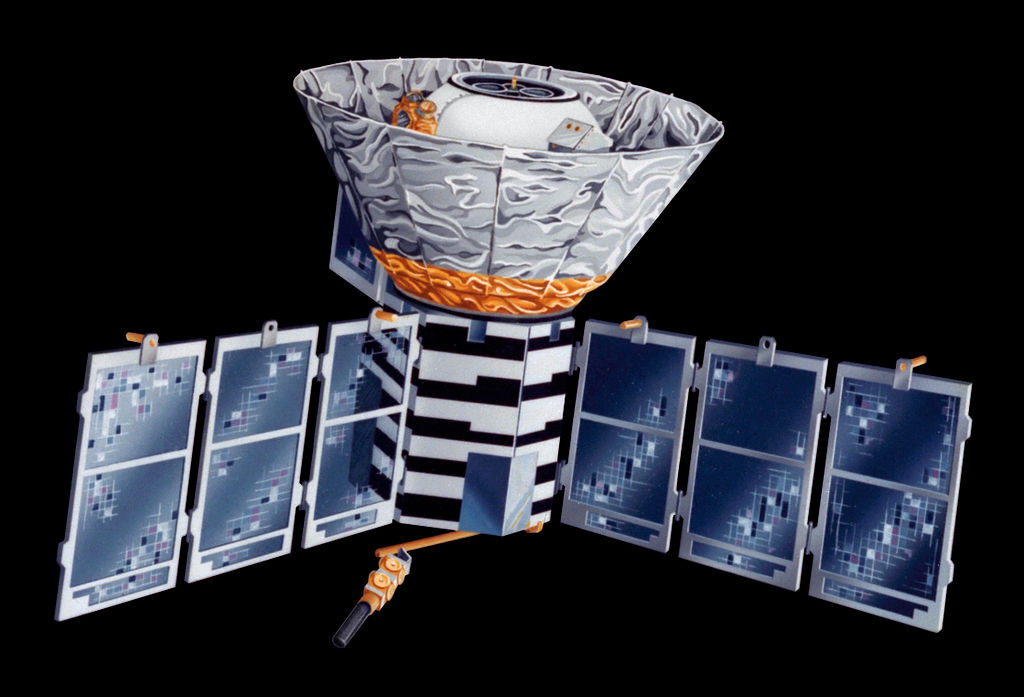
\includegraphics[width=0.8\linewidth]{Figuras/Artigo1/COBE.jpg}
	\caption{Satélite COBE, enviado para o espaço a fim de observar a CMB. Fonte: \href{https://en.wikipedia.org/wiki/List_of_cosmic_microwave_background_experiments\#/media/File:Cobe_vision1.jpg}{Wikipédia}.}
	\label{fig:COBE}
\end{figure}

Depois de sua primeira detecção, a CMB foi estudada por várias outras missões, pois ela é, no sentido mais literal da palavra, uma foto do universo primordial (ver Figura \ref{fig:CMB}). Através dela, podemos realmente fazer ``arqueologia'' com nosso universo e descobrir características que ele tinha há 13,8 bilhões de anos!

Atualmente, a CMB é tema de estudo de diversos pesquisadores no Brasil e no mundo. A quantidade de informação que ela nos dá sobre o universo primitivo é incrível, tanto que daria praticamente um outro texto aqui do Newston. Apenas para mencionar alguns satélites lançados para estudar a CMB, temos o COBE\footnote{\textit{Cosmic Microwave Background Explorer}. Ver Figura \ref{fig:COBE} .}(1989-1990), WMAP\footnote{\textit{Wilkinson Microwave Anisotropy Probe}.}(2001-2010), e Planck (2009-2013).



\mysubtitle{O Plasma Primordial}

Vimos então que, antes da Recombinação, não existiam sequer átomos no universo: os prótons e elétrons eram livres e, quando tentavam se juntar, eram separados por um fóton altamente energético.

Chamamos esse estado da matéria, no qual não há sequer átomos, de \textbf{plasma}. Porém, antes da Nucleossíntese Primordial, nem os núcleos dos átomos existiam. Mais precisamente, os prótons e nêutrons que os constituem estavam quebrados em seus componentes, os quarks e os glúons.

\begin{figure}[H]
	\centering
	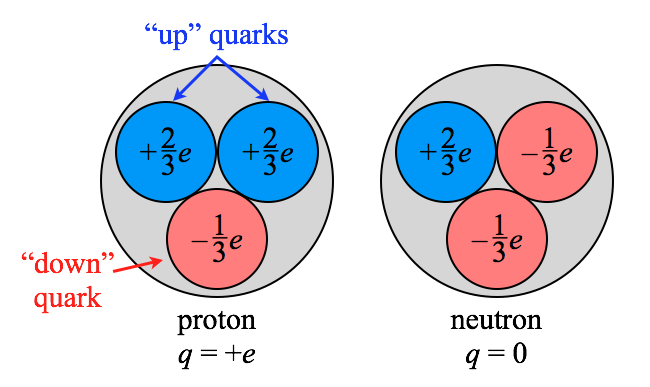
\includegraphics[width=\linewidth]{Figuras/Artigo1/quarks.png}
	\caption{Os prótons e nêutrons são feitos de quarks. Fonte: \href{https://5-volts.blogspot.com/2016/06/carga-eletrica.html}{An Introduction to Electricity and Magnetism}.}
	\label{fig:quarks}
\end{figure}

Chamamos então o estado do universo nessa época de um \textbf{plasma de quarks e glúons}. As outras partículas, como fótons, neutrinos e elétrons também estavam ali, mas o nome é dado porque quarks e glúons livres só ocorrem nesse estado da matéria.

Esse plasma pode então ser descrito como um grande carnaval, com partículas de todas as cores e sabores sambando em um frenezi louco nessa sopa primordial. Esse era o passado do Cosmos.

\mysubtitle{Mais problemas}

Quando observamos a CMB (Figura \ref{fig:CMB}), notamos uma coisa curiosa: ao longo de todo o céu, ela possui em média a mesma temperatura (cerca de 3 Kelvin, ou -270ºC). Isso é muito estranho pois, para que um sistema entre em equilíbrio térmico (atinja uma mesma temperatura), é necessário que diferentes partes dele tenham tido contato. Por exemplo, um cubo de gelo jamais derreterá se não for tirado da geladeira.


No caso da CMB, vemos então que regiões muito afastadas do céu têm a mesma temperatura. Mas elas não tiveram contato térmico: a luz de um lado não interagiu com a do outro lado para que todas tenham a mesma temperatura (ver Figura \ref{fig:horizon}). Esse fato não é bem compreendido pela cosmologia moderna, sendo conhecido como \textbf{Problema do Horizonte}.

Na verdade, há outros mistérios de nosso universo: assumimos que ele é espacialmente plano\footnote{Ele poderia ter curvatura espacial e ser uma 3-esfera, por exemplo}, mas por que haveria ele de ser assim?



Além disso, vemos um universo cheio de estruturas: galáxias, buracos negros, filamentos, planetas, sóis, aglomerados de galáxias, etc. Uma outra pergunta a ser respondida é: daonde vieram tais estruturas? Como elas se formaram?


\begin{figure}[H]
	\centering
	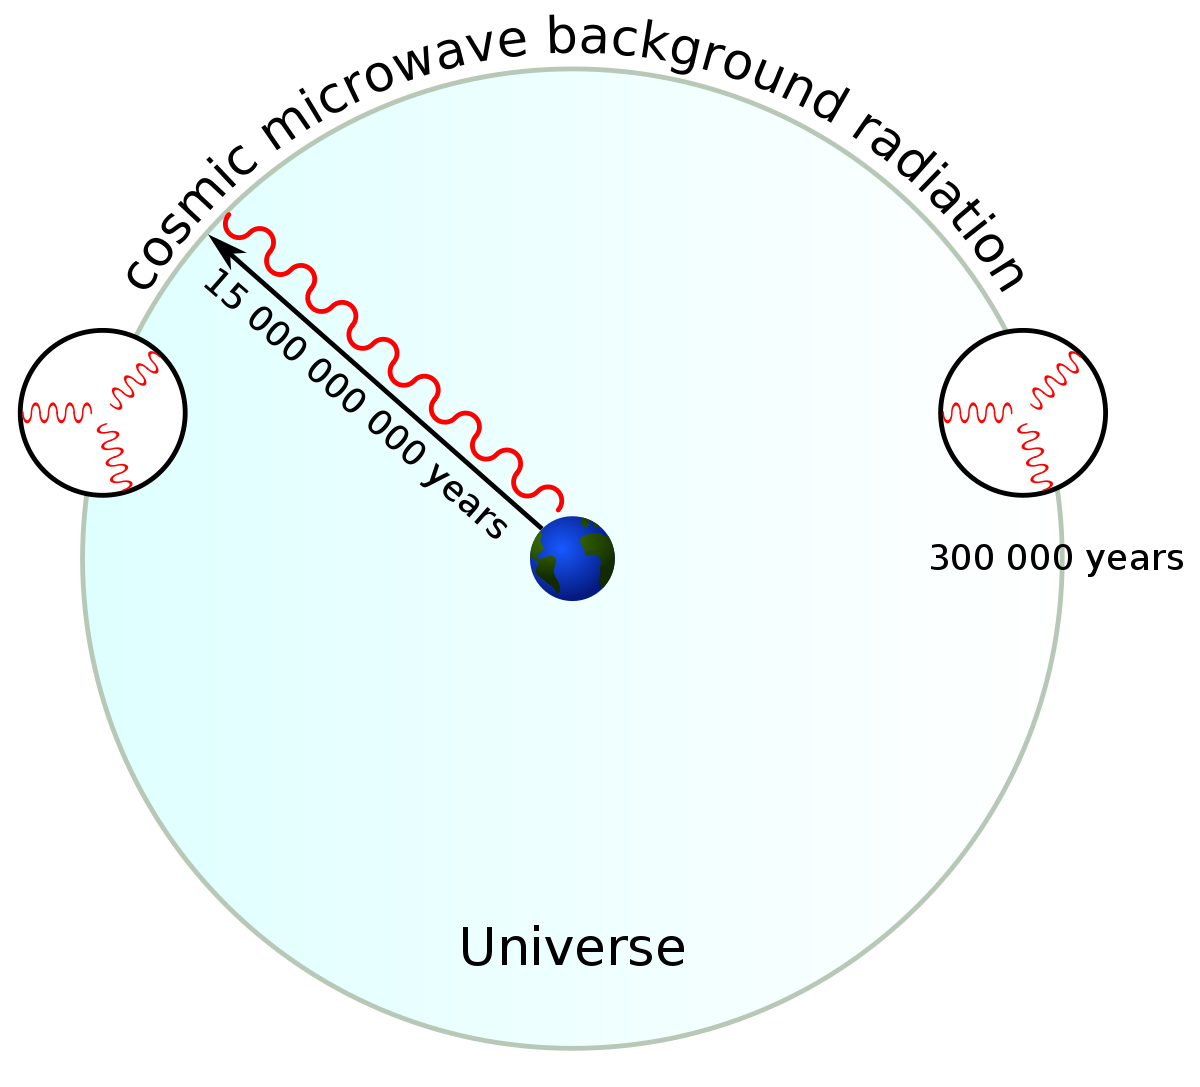
\includegraphics[width=\linewidth]{Figuras/Artigo1/horizon.png}
	\caption{Ao olharmos a CMB, vemos pontos de direções opostas(direita e esquerda) tem a mesma temperatura. Fonte: \href{https://www.pngwing.com/en/free-png-irtdi}{PNGwing}.}
	\label{fig:horizon}
\end{figure}

A resposta é que tais problemas... ainda não têm resposta. Mas há tentativas de resolvê-los. Uma das mais comuns é a chamada \textbf{Inflação}, que modifica a expansão do universo e resolve o problema do Horizonte e os outros em uma única tacada. Veremos isso no próximo texto da coleção: \textbf{Era Inflacionária}, aqui no Newston!

\authorinfo{Luiz Felipe Demétrio}{http://lattes.cnpq.br/3247376940028009}
% Use esse comando para adicionar o nome do autor(a) do artigo no final, e o link para o seu currículo lattes




\end{multicols}

 % Use essa linha d  e comando para adicionar novos artigos (recomenda-se criar um arquivo .tex para cada artigo)
    %\protect\mytitle{À Luz de Caravaggio} % Título do Artigo    
\addchaptersummary{À Luz de Caravaggio}{Sumario/Figs_Sumario/FigArtigo2.jpg}{Nesse artigo, a vida de Michelangelo Merisi, Caravaggio, é apresentada por meio de suas obras, e essas interpretadas pelos olhos da Óptica Geométrica.}{Milena Camila Fernandes} 
\newcommand{\artigodois}{\begin{center}\textcolor{base}{\MakeUppercase{À Luz de Caravaggio}}\end{center}}

\begin{multicols}{2}

Apresentar Michelangelo Merisi da Caravaggio (Caravaggio, 29 de setembro de 1571 — Porto Ercole, 18 de julho de 1610) \ref{ref1:artigo2} não é tarefa simples, tanto pela complexidade da arte quanto do próprio artista. Para isso, ele será retratado aqui por meio dos seus quadros e contextos\footnote{Por muitas vezes, a adjetivação e interpretação de Caravaggio e suas obras presentes nesse artigo --- quando não acompanhadas de fontes científicas --- são feitas através dos olhos da autora do texto, uma simples admiradora de seu trabalho.}. 

\begin{figure}[H]
	\centering
	
\includegraphics[width=0.9\linewidth]{Figuras/Artigo2/m1.jpg}
	\protect\caption{São Mateus e o Anjo. Caravaggio; c. 1602; Óleo sobre tela; 295 cm; (destruído). [Fonte: \href{https://www.wikiart.org/pt/caravaggio}{WikiArt}].}
	\label{fig:m1}
\end{figure}

Como início, podemos mostrar esse maneirista de formação, mas considerado o pai da arte barroca, por meio de duas obras, as quais  tinham o mesmo objetivo: retratar o apóstolo São Mateus e o Anjo para serem colocados na Capela Contarelli da Igreja de São Luís dos Franceses (Roma). A primeira versão da obra (Figura \ref{fig:m1}) foi rejeitada pelos cardeais, isso porque, como podemos notar, a pintura de Caravaggio traz uma proximidade extremamente humana entre o homem e o Anjo, retratando ambos em igualdade, em que o Anjo chega a segurar a mão de São Mateus para o ajudar. Assim, Caravaggio deixa sua essência nessa obra — uma retratação sem idealizações —, mas que seguia o caminho oposto desejado pelos cardeais, tornando-a ``humana demais''  \reftres{ref1:artigo2}{ref2:artigo2}{ref3:artigo2}. Segundo o cardeal Matteo Contarelli, a obra deveria seguir os seguintes requisitos \ref{ref4:artigo2}: 

\textit{``San Matteo na cadeira com um livro, ou volume, como melhor pareça, no qual mostre a escrita ou a vontade de escrever o Evangelho e ao lado dele o Anjo de pé maior do que o natural em acto que pareça de pensar ou noutra atitude.''}

Desse modo, Caravaggio teve que a refazer e o resultado pode ser visto na Figura \ref{fig:m2}. É notável a diferença de proximidade entre o Anjo e São Mateus, dando ao primeiro a santidade necessária exigida pela Igreja, como um ser que desce para fornecer ao humano a inspiração para dar início a sua escrita sagrada, mas que mantém uma distância que caracteriza sua hierarquia, sua importância divida. Essa obra se encontra na \href{https://commons.wikimedia.org/wiki/File:1475RomaSLuigiFrancesiInside.jpg}{capela} até os dias atuais, mas a primeira versão foi destruída num incêndio no final da Segunda Guerra Mundial, restando apenas uma foto da pintura, exibida nesse artigo.

Apesar de ambas as obras terem diferenças em diversos aspectos entre os personagens que as compõem, é certo que elas usam uma técnica em comum: a luz e sombra. Essa técnica já existia na história da arte, mas foi aperfeiçoada por Caravaggio, dando-a um caráter singular: \textbf{o tenebrismo}. Ela consiste em um claro-escuro ainda mais extremado e dramático, em que o uso da luz e sombra é construído para trazer à imagem um realismo psicológico, um estado de espírito que ultrapassa o quadro e atinge nossos sentidos \refdois{ref1:artigo2}{ref7:artigo2}.

\begin{figure}[H]
	\centering
	
\includegraphics[width=0.8\linewidth]{Figuras/Artigo2/m2.jpg}
	\protect\caption{A Inspiração de São Mateus. Caravaggio; c. 1602; Óleo sobre tela; 292 cm × 186 cm; San Luigi dei Francesi, Roma. [Fonte: \href{https://www.wikiart.org/pt/caravaggio}{WikiArt}].}
	\label{fig:m2}
\end{figure}

Nesse viés, escuros profundos ao fundo na tela complementam uma luz extremamente vívida em pontos  estratégicos — como nos rostos, iluminando a expressão dos personagens ou evidenciando algum movimento, como se um refletor estivesse acima da figura \ref{ref1:artigo2}. Tais pontos foram milimetricamente concebidos para que os detalhes nos saltassem os olhos e transmitissem algum tipo de sentimento.  
	
A segunda versão da ``A Inspiração de São Mateu'' está na Capela Contarelli, com mais duas obras de Caravaggio que seguem a mesma técnica e temática. À esquerda dessa obra, encontra-se ``O Chamado de São Mateus'' (Figura \ref{fig:m3}) e, ao observá-la, podemos perceber uma fonte de luz que entra pela janela e toca em pontos importantes da tela. A mão de Jesus é meticulosamente iluminada e faz luz a seu movimento, apontando para São Mateus. Esse também tem sua expressão com muita luz — e, em conjunto, a sua mão —, para que seja possível enxergar os detalhes psicológicos que a tela tem a transmitir, como esse gesto simbólico que, segundo o Professor Giovanni Bagnoli ``[...] transforma o pecador em apóstolo [...]'' \refdois{ref2:artigo2}{ref3:artigo2}.
A obra continua com um fundo escuro e com ausência de luz em personagens ``secundários''\footnote{A palavra ``secundários'' foi utilizada para denotar os personagens que estão para além do significado religioso que ela deveria ter, como por exemplo o homem que conta moedas, ao canto da mesa, o qual foi considerado um autorretrato de Caravaggio.} do cenário, como no rosto de Pedro, que segura Jesus, em que apenas a sua mão tem maior enfoque. 

Para completar a tríade de uma parte da Capela, temos ``O Martírio de São Mateus'' (Figura \ref{fig:m4}), obra à direita da ``Inspiração de São Mateus''. Nesse trabalho, podemos ver um carrasco no centro da composição, com o apóstolo Mateus deitado. No entorno, existem muitas figuras expressivas típicas do barroco\footnote{Na pintura, escultura, arquitetura e artes decorativas, estilo, com elementos do alto Renascimento e do Maneirismo e ligado à estética da Contrarreforma, nascido em Roma c1600 e cujas características básicas são o dinamismo do movimento com o triunfo da linha curva e (esp. na escultura e pintura) a busca da captação das reações emocionais humanas. Cedo internacionalizado, o estilo ganhou traços específicos em cada país \ref{ref6:artigo2}.}. Nessa situação, a luz dá foco ao movimento dos dois personagens ``principais'', à movimentação do carrasco que dará um golpe fatal no apóstolo e à proteção que São Mateus tenta manter com um gesto de defesa\footnote{Nessa obra, é comprovado que o homem no fundo da tela, olhando diretamente para ``nós'', é um autorretrato de Caravaggio.}.

Olhando o tenebrismo pelo viés da Física, podemos entender melhor como usar o claro-escuro pela compreensão de alguns conceitos da óptica geométrica no que se refere ao que é luz, sombra e penumbra. Inicialmente, a fonte de luz que incidirá sobre o objeto pode ser de origem primária --- gera sua própria luz, como o Sol ---, ou de origem secundária, que necessita que uma fonte de luz primária reflita no objeto para que ele seja visto, como a Lua. Uma vez que a fonte emite luz, ela pode encontrar um objeto que é opaco, transparente ou translúcido. Para o primeiro, a luz é absorvida e refletida e não é possível que ela o atravesse. Já o segundo é um objeto que permite a passagem de luz sem que ela sofra desvios e, por fim, no terceiro caso é permitida a passagem de luz, mas ela sofre desvios e o observador não consegue enxergar a imagem com nitidez. 

\end{multicols}

\begin{figure}[H]
    \centering
	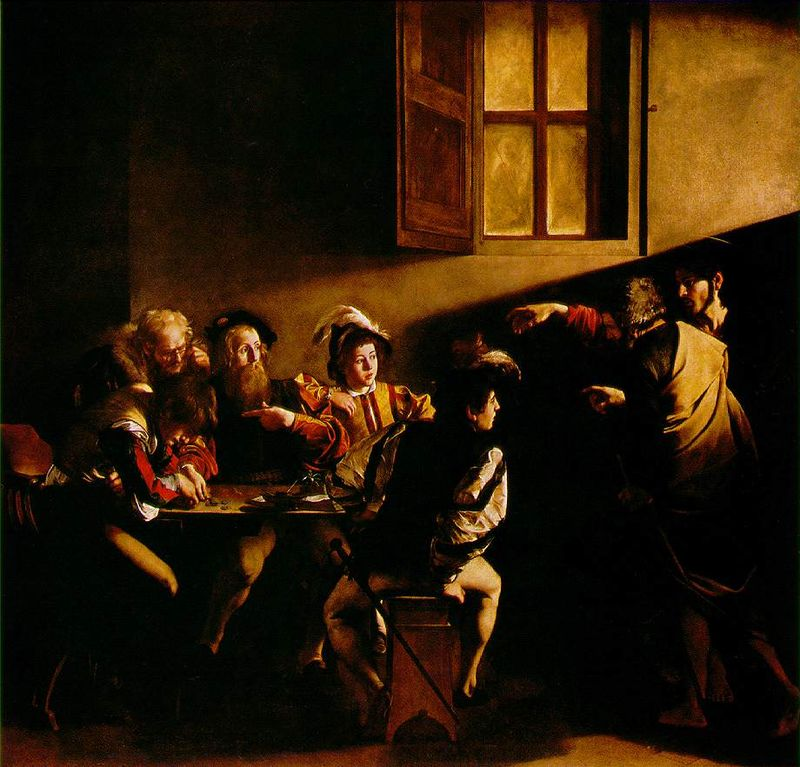
\includegraphics[width=0.7\linewidth]{Figuras/Artigo2/m9.jpg}
	\protect\caption{Vocação de São Mateus. Caravaggio; c. 1599-1600; Óleo sobre tela; 340 cm × 322 cm; San Luigi dei Francesi, Roma. [Fonte: \href{https://www.wikiart.org/pt/caravaggio}{WikiArt}].}
    \label{fig:m3}
\end{figure}

\begin{multicols}{2}


Paralelo a isso, a junção da fonte, objeto e anteparo (ou observador) obedecerá o Princípio da Propagação Retilínea da Luz\footnote{O Princípio da Independência dos Raios Luminosos e o Princípio da Reversibilidade dos Raios Luminosos também se fazem presente nos conceitos de luz e sombra, mas não foram abordados neste artigo. Todos podem ser melhor compreendidos em \ref{ref4:artigo2}.}, isto é, a luz se propaga em linha reta nos meios homogêneos, transparentes e isotrópicos. Como consequência, temos a produção de sombra (ausência total de luz) atrás de objetos opacos, para os casos em que a fonte é puntiforme, e também a produção de sombra e penumbra (ausência parcial de luz) quando a fonte é extensa \refdois{ref8:artigo2}{ref9:artigo2}.

Nas obras apresentadas neste artigo, é possível identificar que as técnicas utilizadas seguem os preceitos apresentados acima. Na Figura \ref{fig:m2}, a luz incide acima (e lateralmente) de São Mateus e produz sombra em lugares nos quais ela previamente encontrou um objeto que a absorveu e refletiu. Isso pode ser observado, por exemplo, abaixo do apóstolo, nos detalhes do seu pé, nas dobras de suas vestimentas e no peito do Anjo. Em conjunto, é possível notar que, em cada detalhe da tela os princípios são respeitados, como o da trajetória retilínea da luz nas curvaturas dos braços do Anjo. 
\end{multicols}

\begin{figure}[H]
	\centering
	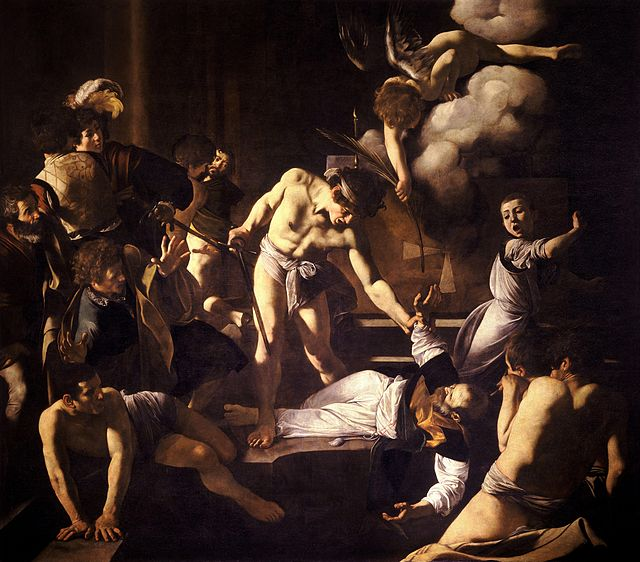
\includegraphics[width=0.7\linewidth]{Figuras/Artigo2/m7.jpg}
	\protect\caption{O Martírio de São Mateus. Caravaggio; c. 1599-1600; Óleo sobre tela; 323 cm × 343 cm ; San Luigi dei Francesi, Roma. [Fonte: \href{https://www.wikiart.org/pt/caravaggio}{WikiArt}].}
	\label{fig:m4}
\end{figure}

\begin{multicols}{2}
    
O mesmo ocorre com as Figuras \ref{fig:m3} e \ref{fig:m4}. Na primeira, vale ressaltar o enfoque que o Caravaggio dá às mãos de Jesus, Pedro e Mateus, evidenciando o objetivo da cena. Já na segunda, é nítida a percepção dos dois elementos centrais da tela, iluminados por uma fonte lateral que permite que as expressões do carrasco e de São Mateus sejam evidenciadas, mesmo que seus rostos não estejam totalmente visíveis. 
	
A três obras apresentadas aqui ainda estão expostas na Capela Contarelli, como apresentado na Figura \ref{fig:m5}. Essas e outras várias do artista fazem uso do tenebrismo, técnica que revolucionou o teatro, o cinema, a pintura e a fotografia. Até os dias atuais, sua influência no uso da luz e sombra se faz presente em todas essas expressões artísticas\footnote{E certamente em muitas outras que não foram citadas aqui.}. 
	
É evidente que, com a morte de Michelangelo Merisi, com apenas 38 anos, a história da arte perdeu um de seus maiores gênios que concedeu à humanidade uma coleção de obras monumentais, em tamanho e expressividade, que nunca deixarão de ter influência na arte e todos os seus vieses. Seu divino claro-escuro o faz eternamente vivo. 

\begin{figure}[H]
	\centering
	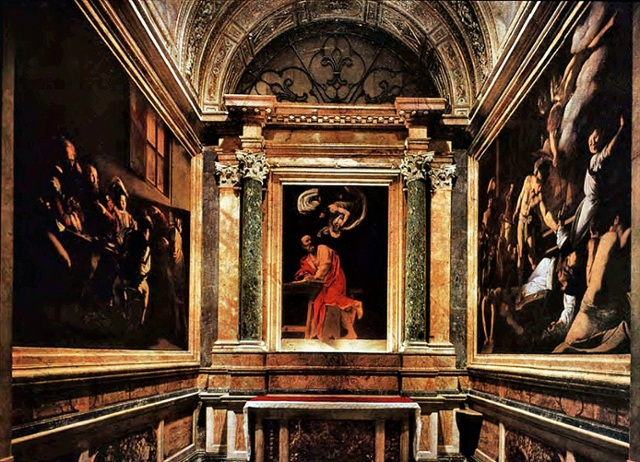
\includegraphics[width=0.95\linewidth]{Figuras/Artigo2/m8.jpg}
	\protect\caption{Capela Contarelli da igreja de S. Luís dos Franceses, em Roma, com as três pinturas de Caravaggio. [Fonte: \href{https://pt.wikipedia.org/wiki/A_Inspira\%C3\%A7\%C3\%A3o\_de\_S\%C3\%A3o\_Mateus\#/media/Ficheiro:1475RomaSLuigiFrancesiInside.jpg}{WikiArt}].}
	\label{fig:m5}
\end{figure}

\noindent\textit{``Não sou um pintor valentão, como me chamam, mas sim um pintor valente, isto é, que sabe pintar bem e imitar bem as coisas naturais.''}\\
	Michelangelo Merisi, dito Caravaggio.

\authorinfo{Milena Camila Fernandes}{http://lattes.cnpq.br/3118223351391736}

\end{multicols}



    % Decidimos remover o artigo 2 para que o limite de compilação do Free Trial do Overleaf não seja excedido para usuários gratuitos
    \protect\mytitle{Tipos de radiações}    
\addchaptersummary{Tipos de radiações}{Sumario/Figs_Sumario/FigArtigo3.jpg}{Entenda o que é radiação, como se classificam e conheça algumas de suas aplicações, bem como a importância dos materiais de blindagem de radiação!}{Murilo Aparecido da Silva} 
\newcommand{\artigotres}{\begin{center}\textcolor{base}{\MakeUppercase{Tipos de radiações}}\end{center}}

\mytitlesubtitle{e a importância de materiais para blindagem contra radiação}  

\begin{multicols}{2}

\mysubtitle{Primeiros Contatos}

A história da radiação teve seu início com as descobertas de Wilhelm K. Röntgen (Figura \ref{fig:RontgenBecquerel}), em 1895. Em suas pesquisas sobre a propagação de raios catódicos, ele havia produzido radiação eletromagnética no comprimento de onda dos raios X. Tal feito possibilitou a outros cientistas o início de mais pesquisas sobre radiações, como é o caso de Henri Becquerel (Figura \ref{fig:RontgenBecquerel}), que estudou as características de substâncias fosforescentes e fluorescentes, além das propriedades de sais de urânio que o levaram à descoberta da radioatividade.

\begin{figure}[H]
			\centering
			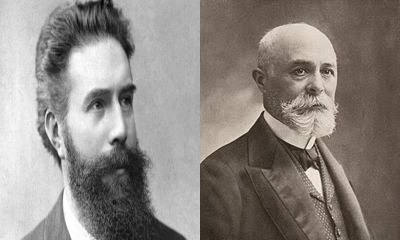
\includegraphics[width=\linewidth]{Figuras/Artigo3/Rontgen_e_Becquerel.png}
			\caption{Wilhelm K. Röntgen (à esquerda) [Fonte: \href{https://www3.unicentro.br/petfisica/2018/03/02/wilhelm-conrad-rontgen-1845-1923/}{Unicentro Pet Física}] e Henri Becquerel (à direita) [Fonte: \href{https://www3.unicentro.br/petfisica/2017/06/22/antoine-henri-becquerel-1852-1908/}{Unicentro Pet Física}].}
			\label{fig:RontgenBecquerel}
\end{figure}

Procedendo os trabalhos iniciados por Becquerel, o casal Marie e Pierre Curie (Figura \ref{fig:MarieEPierre}) descobriu outros dois elementos químicos que também eram capazes de emitir radiação:  Rádio (Ra) e Polônio (Po) \refdois{ref1:artigo3}{ref2:artigo3}.

\mysubtitle{O que é radiação? Como se classificam? Quais suas aplicações?}

Radiações são ondas eletromagnéticas ou partículas que se propagam com uma determinada velocidade. Possuem energia e cargas elétrica e magnética, podendo ser geradas por fontes naturais ou por dispositivos construídos pelo homem. Elas apresentam energia variável desde valores pequenos até muito elevados \reftres{ref1:artigo3}{ref2:artigo3}{ref7:artigo3}.

\begin{figure}[H]
			\centering
			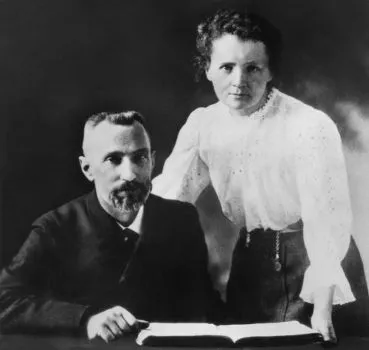
\includegraphics[width=\linewidth]{Figuras/Artigo3/Marie & Pierre Curie.png}
			\caption{Marie e Pierre Curie. [Fonte: \href{https://brasilescola.uol.com.br/quimica/maria-curie-descoberta-radioatividade.htm}{Brasil Escola}].}
			\label{fig:MarieEPierre}
\end{figure}


As radiações eletromagnéticas mais conhecidas são: luz, micro-ondas, ondas de rádio, radar, laser, raios X e gama. As radiações sob a forma de partículas – com massa, carga elétrica e carga magnética – mais comuns são os feixes de elétrons, os feixes de prótons, a radiação beta e a radiação alfa \ref{ref7:artigo3}.

Devido ao seu amplo intervalo energético, uma radiação pode ser descrita como não ionizante ou ionizante a depender de sua energia, o termo ionização dá nome ao processo pelo qual um átomo ou molécula adquire carga negativa ou positiva ao ganhar ou perder elétrons, esse processo pode se dar por meio da colisão entre partículas como ilustra a Figura \ref{fig:ProcessoIonizacao}. 



	
As \textit{radiações não ionizantes}, por exemplo, possuem consideravelmente baixa energia e baixa frequência, obedecendo assim a Lei de Planck $E=h\nu$, sendo o tipo de radiação mais presente em nosso dia a dia. Alguns casos particulares são o calor, ondas de rádio e a luz, todas formas de radiação não ionizante. Sem este tipo de radiação não poderíamos apreciar um programa de TV em nossas casas ou cozinhar em um forno micro-ondas \refdois{ref1:artigo3}{ref2:artigo3}.

\begin{figure}[H]
			\centering
			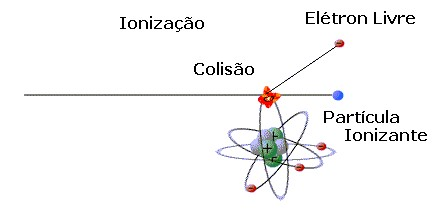
\includegraphics[width=0.9\linewidth]{Figuras/Artigo3/ionização.jpg}
			\caption{Diagrama esquemático do processo de ionização. [Fonte: \href{https://www.fisica.net/aplicada/biofisica/radiacao.php}{física.net}].}
			\label{fig:ProcessoIonizacao}
\end{figure}



Já as \textit{radiações ionizantes} são um tipo de radiação menos presente em nosso cotidiano habitual: é um tipo de radiação que possui altos níveis de energia e altas frequências quando comparadas às radiações não ionizantes. De forma geral, as radiações ionizantes são aquelas que têm energia suficiente para provocar ionização em átomos e moléculas, tornando eletricamente carregado o meio físico em que penetra. Seus efeitos podem ser danosos para as células, afetando o material genético e causando doenças graves, como o câncer. Alguns tipos de radiação ionizante são as partículas alfa e beta, os raios gama e os raios-X \ref{ref1:artigo3}. 



\end{multicols}

\begin{figure}[H]
            \centering
			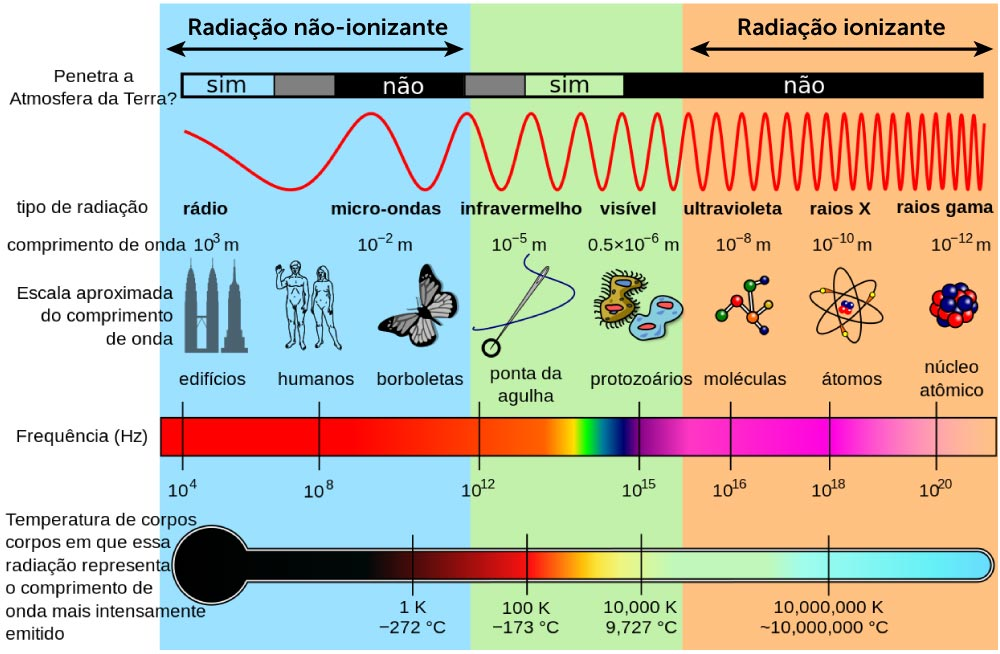
\includegraphics[width=0.9\linewidth]{Figuras/Artigo3/radiacao.jpg}
			\caption{Diagrama esquemático dos tipos de radiações. [Fonte: \href{https://www.sapralandauer.com.br/protecao-radiologica-saiba-sobre-os-principais-aspectos-normas-e-tecnologias-empregadas/o-que-e-radiacao-nocoes-basicas-de-protecao-radiologica/\#toggle-id-2}{Sapralandauer}].}
			\label{fig:DiagramaEsq}
\end{figure}

\begin{multicols}{2}

Suas principais aplicações se dão nas área de saúde - em radiografias, tomografias, exames de densitometria óssea, entre outros - e alimentícia (...), matando micro-organismos presentes em frutas, verduras e legumes, fazendo com que durem mais tempo e sejam mais saudáveis para o consumo \ref{ref8:artigo3}.

Na Figura \ref{fig:DiagramaEsq}, está um diagrama esquemático dos tipos de radiação, sua frequência, e uma escala aproximada de seu comprimento de onda.

\mysubtitle{Materiais para blindagem contra radiação ionizante}

Devido ao perigo que as radiações ionizantes podem nos oferecer, ao longo das décadas diferentes materiais para proteção contra elas foram produzidos a fim de proteger os seres humanos e seus arredores de seu impacto destrutivo \ref{ref8:artigo3}.

Os materiais utilizados para tal finalidade devem possuir alta densidade a fim de se alcançar uma forte habilidade de blindagem. Por esse motivo, são comumente usados materiais como o chumbo e o concreto.

Entretanto, materiais livres de chumbo têm ganhado nos últimos anos notória apreciação por parte dos pesquisadores, pois o chumbo é um material tóxico. Assim muitas pesquisas visam propor novos materiais que não possuem toxicidade como meio de blindagem. 

Em especial, pode-se citar os vidros livres de chumbo, que, por possuírem boa transparência à luz visível e, mais importante ainda, sua composição, espessura e densidade pode ser alterada e controlada durante o processo de preparação. Isso os credencia como um material promissor para o desenvolvimento de diferentes tipos de equipamentos de proteção contra radiação, como protetores faciais e janelas de salas de raios X \ref{ref9:artigo3}.

Tendo em vista tudo que foi apresentado, temos, mesmo que de forma sucinta, a percepção do que é radiação e a importância de seu uso e aplicações em nosso mundo. Também entendemos a importância dos materiais utilizados em proteção radiológica, pois a radiação ionizante, mesmo sendo tão benéfica nos mais diversos meios, ainda pode nos ser prejudicial à saúde. Por isso, temos que ter em vista a importância de seu uso controlado e a utilização de equipamentos que visem a nossa proteção quando necessário seu uso. Vimos também a importância da pesquisa de materiais que não sejam tóxicos, buscando assim por novas substâncias que não sejam prejudiciais à nossa saúde.

\authorinfo{Murilo Aparecido}{http://lattes.cnpq.br/2055729643800351}




\end{multicols}
    \protect\mytitle{A Física dos Esportes}    
\addchaptersummary{A Física dos Esportes}{Sumario/Figs_Sumario/FigArtigo4.jpg}{Na cabeça de muitos, Física e Esportes nunca andaram lado a lado, mas a grande verdade é que eles tem tudo a ver. Você pode achar que não, mas já fez muita conta de cabeça numa partida de futebol!}{Vítor Hugo Ribeiro} 
\newcommand{\artigoquatro}{\begin{center}\textcolor{base}{\MakeUppercase{A Física dos Esportes}}\end{center}}

\begin{figure}[H]
		\centering
		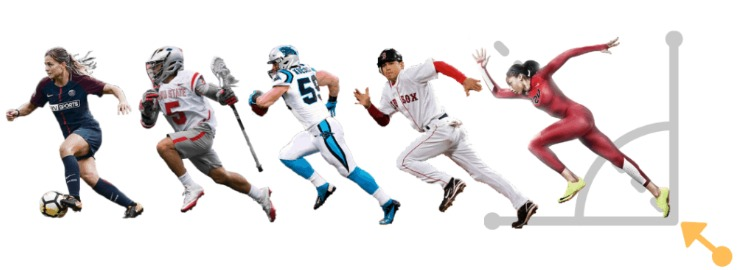
\includegraphics[width=0.95\linewidth]{Figuras/Artigo4/esportes.jpeg}
		\caption{As leis Físicas estão presentes, sem exceção, em todos os esportes. [Fonte:  \href{https://velocityspusa.com/myth-or-fact-speed-training-is-sport-specific/}{velocityspusa}].}
		\label{fig:v1}
	\end{figure}

\begin{multicols}{2}

A história da Física se inicia na antiguidade, quando as pessoas, por algum motivo, começaram a se perguntar os ``porquês'' das coisas. Ou melhor ainda, falando isso de uma maneira um pouco mais específica, começaram a se perguntar a respeito da natureza e suas interações, tentando entender os conceitos por trás destes elementos, sem que houvesse a necessidade de algo místico para explicá-los. E agora, no momento atual, você deve estar se perguntando o que isso tem a ver com o título desse texto, visto que eu sequer citei o termo ``Esporte'' nessa introdução. Pois bem, respondendo a sua pergunta, é interessante começar com essa introdução histórica pois foram nesses momentos iniciais da Física que surgiram os primeiros pensamentos a respeito do movimento e de como descrevê-lo. Nesse contexto, também não existe palavra melhor para se referir aos esportes do que movimento. Esportes são caracterizados por seres em movimento e a Física foi a primeira ciência que se preocupou em estudá-los.
 
Apesar dessa relação intrínseca entre os termos Física e Esportes para com a palavra movimento, hoje em dia não se vê uma conexão direta entre os três. Na verdade, o que podemos notar é uma relação um tanto quanto oposta, demonstrada no fato de que muitos alunos, no geral, preferem as aulas de Educação Física do que as de Física ou Matemática. É claro que esse tipo de comparação não é justa, visto que diversos outros fatores interferem nessa escolha, mas o ponto principal que pretendo trazer aqui é que dificilmente as pessoas associam os esportes com pensamentos e conceitos Físicos. Nos esportes, tudo é mais dinâmico e intuitivo, não é necessário fazer cálculos para se chegar a um resultado e, por isso, talvez, a aula de Educação Física seja a preferida. No entanto, ao mesmo tempo, realizar um determinado movimento exige preparação física e psicológica para que ele seja executado da maneira correta. Dessa forma, pode até não parecer, mas isso exige diversos raciocínios físicos e aproximações que são calculadas de maneira instintiva e que culminam naquele golaço do camisa 10 no gol do time adversário. 
 Talvez seja exatamente por não enxergar esse tipo de relação, que as pessoas sintam um pouco de medo da Física e achem-na muito difícil. Quando se fala nesta disciplina, todo mundo se lembra das equações que estudava, ou na verdade, lembram que havia muitas equações, mas dificilmente se lembram dos conceitos por trás delas. Ideias como força e velocidade são comuns no nosso dia a dia e, no geral, todo mundo sabe ou tem uma noção mínima do que significam. Porém, quando partimos para conceitos como potência e trabalho, altamente relacionados com atividades esportivas, as pessoas não têm ideia de como explicá-los, embora cheguem a discutir ideias relacionadas a eles quando veem o movimento de um atleta numa modalidade olímpica. Além disso, ao realizar tal análise, as pessoas lidam com situações muito mais complicadas do que aquelas estudadas nas aulas de Física, em que o atrito era desprezível e todo o resto constante. Quando avaliamos uma situação na realidade, assim como nos esportes, nada é constante, ou melhor ainda, tudo está em constante mudança. Nesse sentido é um tanto quanto interessante observar que as pessoas sentem mais interesse em estudar uma situação complicada como esta do que uma situação simples como aquelas abordadas em salas de aula. Mas aqui, novamente, diversos fatores devem ser levados em consideração para justificar esse tipo de escolha. Talvez o mais importante deles é que nestas discussões a matemática não é a ferramenta principal, mas somente um guia que nos ajuda a ter uma noção de proporção, encaminhando a análise para algo que faça sentido. A nossa capacidade de avaliar proporções diretas ou indiretas e relacioná-las com aproximações torna tudo isso mais simples e configura o cerne dessa nossa conversa.
    
Para trabalhar um pouco disso, vamos revisar estes conceitos e ver como estas ideias se aplicam de maneira prática. Uma forma interessante de fazer isso é realizando a análise de duas modalidades olímpicas muito parecidas, mas também, ao mesmo tempo, muito diferentes: os $100$m rasos e a maratona. Numa corrida, tudo que citamos está sendo aplicado: velocidade, força, trabalho, potência e ainda algumas coisas a mais. Porém vamos focar nestes 4 primeiros. Os alvos de nosso estudo serão os dois medalhistas de ouro que venceram as modalidades de Maratona e $100$m rasos na Olimipíada do Rio de Janeiro, em 2016. Enquanto, na primeira modalidade, o corredor percorre uma distância total de $42$km, na segunda, o velocista percorre $100$m. Em ambas o objetivo é o mesmo: chegar primeiro. Porém, podemos ver de maneira nítida a diferença entre as duas: a primeira apresenta uma distância a ser percorrida que é $420$x maior que a segunda.

Os dados que vamos utilizar serão apenas três: a distância da prova, o tempo em que essa distância foi percorrida e a energia gasta para percorrê-la. Veja abaixo os dados de cada modalidade:


\begin{figure}[H]
    \centering
    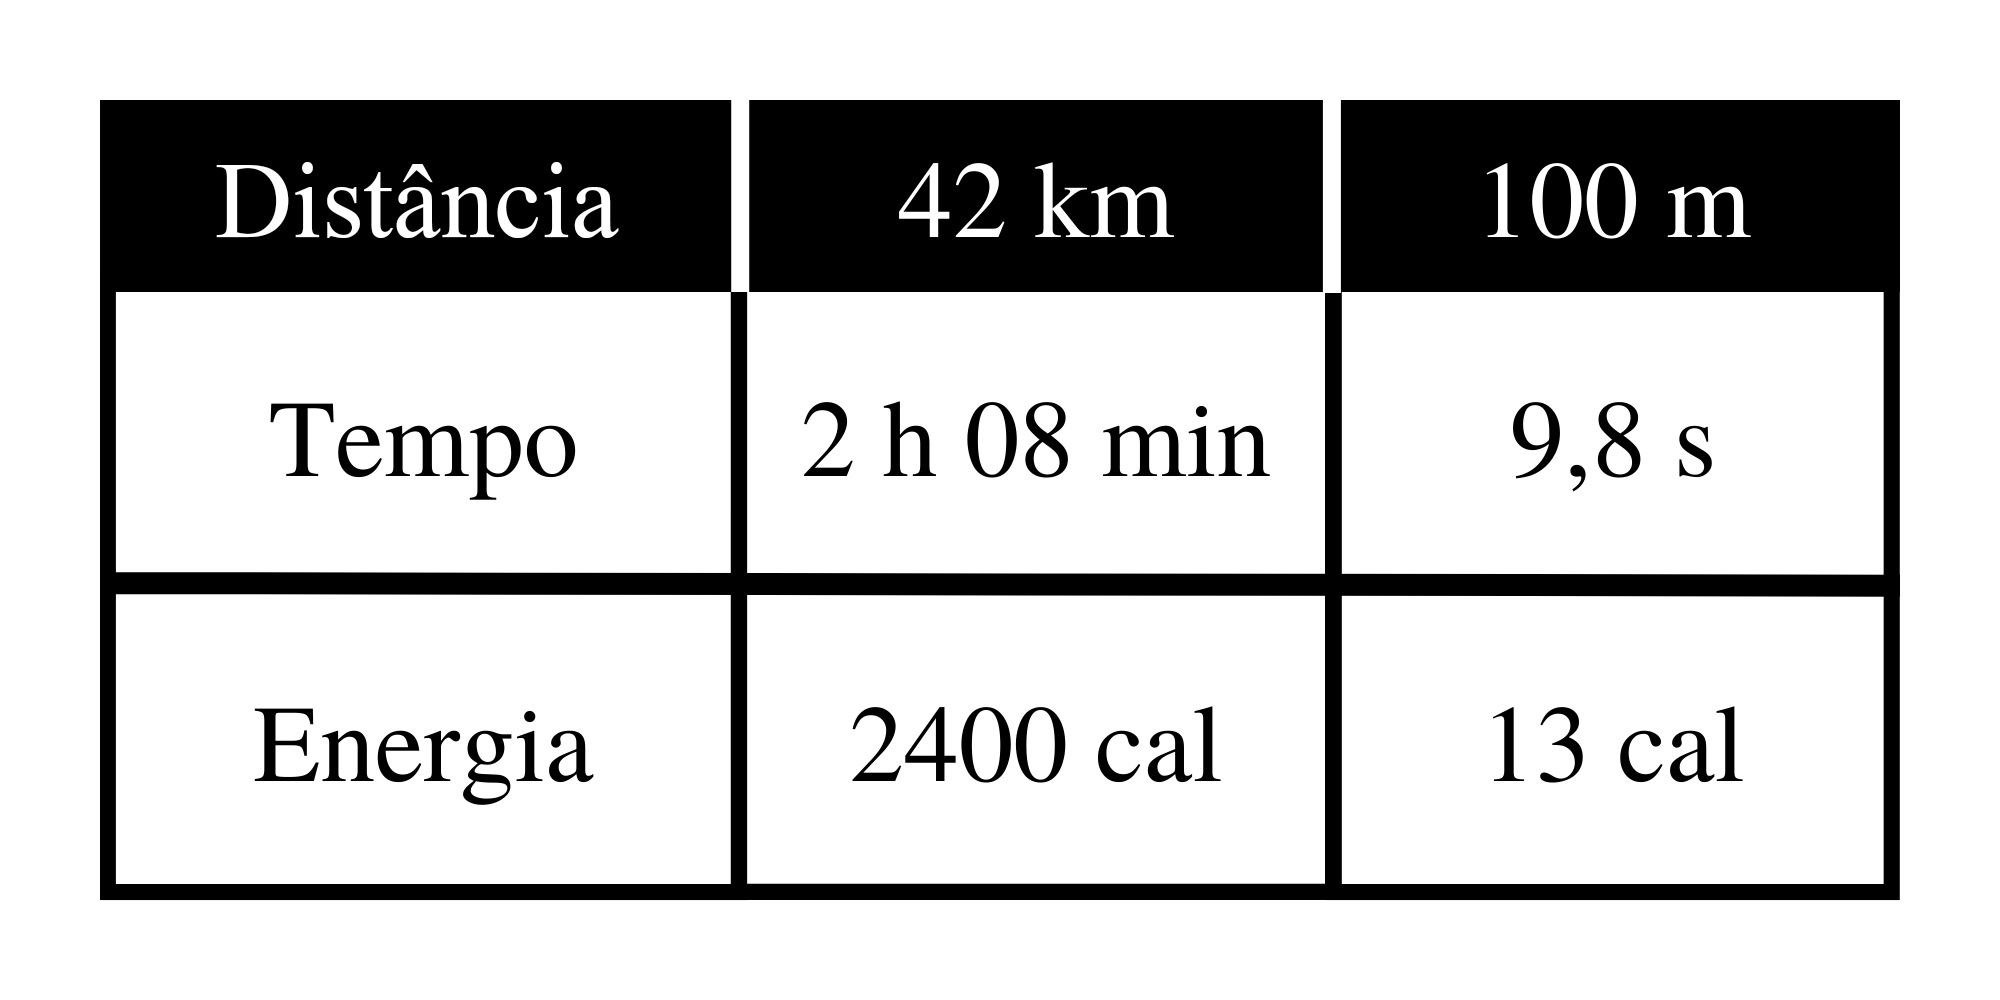
\includegraphics[width=\linewidth]{Figuras/Artigo4/tabela.jpg}
    \caption{Tais dados levam em conta estimativas de gastos calóricos que não correspondem de maneira exata com a realidade, mas que servem como uma forma de aproximação mais do que suficiente para realizarmos nossos cálculos.}
    \label{corredores}
\end{figure}

Tendo essas informações em mãos, podemos começar nossa análise. Primeiramente, iremos avaliar cada ponto utilizando como base nossa intuição e bom senso, para depois confirmarmos essa ideia através de alguns cálculos matemáticos. Essa pode até parecer uma prática simplista, visto que nessa etapa não utilizaríamos nenhum conceito complexo para chegar a conclusão final. Mas a ideia é exatamente essa, tentar chegar a uma conclusão apenas utilizando nossas noções básicas do mundo que nos cerca.

O primeiro tópico a ser estudado será a velocidade, ou seja, pretendemos avaliar a rapidez com que os dois atletas completam a prova e chegar a conclusão de qual deles apresenta uma maior velocidade. Nesse ponto, não é segredo pra ninguém que, de longe, o velocista que percorre apenas $100$ m apresentará uma velocidade muito maior que o maratonista. Não há uma justificativa direta para isso, de maneira que possamos escrevê-la aqui, apenas o bom senso. Uma forma de afirmar esse resultado pode ser dado observando alguns vídeos e comparando o ritmo de corrida de ambos os atletas. Agora, para confirmar essa análise por meios matemáticos, façamos o cálculo da velocidade média deles ao longo da prova. Para isso, aplicaremos uma equação, que é um tanto quanto intuitiva, e suas devidas conversões:

\begin{equation*}
    V_{m} = \dfrac{\text{distância}}{\text{tempo}}
\end{equation*}

\noindent\textbf{Maratonista:}\par % Use \par para criar um novo parágrafo, que é o equivalente explícito de deixar uma linha em branco. Evitando assim o erro underfull \hbox que ocorre quando o compilador não consegue ajustar o texto de forma ideal dentro de uma caixa horizontal

$V_m = \dfrac{42 \: \: \text{km}}{2\: \text{h} \: 08 \: \text{min}} \approx  5,5$ m/s

\noindent\textbf{Velocista:}\par

$V_m = \dfrac{100 \text{m}}{9,8} \approx 10,2$ m/s

Perceba que os dois resultados foram bem diferentes, como era de se esperar, e também concordaram com a análise prévia que havíamos feito. Enquanto o maratonista corre com uma velocidade de cerca de $5,5$ m/s o velocista corre com uma velocidade que é praticamente o dobro daquela apresentada pelo maratonista.

Seguindo por essa linha de raciocínio, podemos utilizar este resultado e inferir a força que cada atleta deve aplicar através dos músculos para alcançar essa velocidade. Tal ideia pode vir com um argumento muito simples: como o corredor de $100$ m rasos atinge uma velocidade maior em menos tempo, provavelmente ele deve fa zer muito mais ``força nas pernas'' para alcançar tal velocidade. Nesse caso, para realizar o cálculo matemático e comprovar, ou não, a nossa análise, utilizaremos uma pequena aproximação. Levaremos em conta que o tempo necessário para o velocista atingir sua velocidade máxima seja de aproximadamente $4,5$ s, ou seja, pouco menos de metade do tempo da prova. Agora, perceba, que não podemos utilizar o mesmo intervalo de tempo para o maratonista, visto que o mesmo não tem a necessidade de acelerar tudo de uma vez logo no começo. Por isso, para fins de aproximação, consideraremos que o maratonista terá cerca de $3$ min para alcançar sua velocidade de prova. Então, utilizando a equação para calcular a aceleração média esses atletas no intervalo de tempo escolhido, temos os seguintes resultados:

\begin{equation*}
    A_{m} = \dfrac{\text{velocidade}}{\text{tempo}}
\end{equation*}

\noindent\textbf{Maratonista:}\par

$A_m = \dfrac{5,5 \: \: \text{m/s}}{3 \: \text{min}} \approx  0,03$ m/$\text{s}^2$

\noindent\textbf{Velocista:}\par 

$A_m = \dfrac{10,2 \text{m/s}}{9,8 \: \text{s}} \approx 1,04$ m/$\text{s}^2$

Ou seja, como podemos observar, a aceleração do velocista é quase $35$x maior do que a aceleração do maratonista. O que, quando colocado em termos de força, que de acordo com a Segunda Lei de Newton é calulada como sendo a massa multiplicada pela aceleração, obteríamos o seguinte:

\noindent\textbf{Maratonista:}\par

$F = (60 \: kg) \times  0,03$ m/$\text{s}^2$ = $1,8 \: N$

\noindent\textbf{Velocista:}\par

$F = (80 \: kg) \times  1,04 $ m/$\text{s}^2$ = $83,2 \: N$

Nesse ponto, também fizemos uma pequena aproximação nas massas de cada atleta, mas veja que o nosso resultado continuou o mesmo. O velocista de $100$m rasos executa uma força muito mais intensa para alcançar o final da prova do que o corredor de maratona. Mas aqui, vale uma ressalva muito grande. Perceba que eu falei ``força muito mais intensa'', me referindo somente ao valor da força que foi aplicada no momento da aceleração. Mas quando falamos do corpo humano, para que ele permaneça em movimento, as pernas precisam continuar executando força. Assim, enquanto após os $9,8$ s de prova do velocista ele pode parar e descansar, o maratonista, por sua vez, precisa continuar aplicando sua força para permanecer em movimento, e pior ainda, um movimento de mais de $2$ horas.

Essa grande diferença no tempo de aplicação de uma força nos conecta diretamente ao quarto conceito que será abordado nessa revisão, o conceito de Potência. Porém, antes de chegar até ele, precisamos ter uma ideia do que significa Trabalho. Na Física, de maneira simples, Trabalho nada mais é do que a energia gasta para realizar um determinado movimento. Em nosso caso, tal conceito está relacionado a quantidade de calorias gastas pelo atleta para completar a prova em questão. Nesse caso, não sobra muito espaço para realizarmos uma análise inicial, visto que estes valores já foram dados previamente. Porém, isso ainda deve fazer sentido para nós que estamos estudando as duas situações. Enquanto o velocista realiza sua prova em menos de $10$ s, o maratonista passa cerca de $2$ horas correndo e, se deixarmos o ``bom senso'' nos guiar, facilmente poderíamos afirmar que o maratonista gasta mais energia para correr ao longo de sua prova do que o velocista. Ainda, nesse ponto, também não há um cálculo que confirme isso, já que pela informação da tabela já possuímos exatamente o valor associado ao trabalho. Logo nesse caso, nos demos bem.

Por fim, abordando agora o quarto conceito, podemos relacionar a discussão exercida quando falamos de força com a ideia de trabalho. No contexto que estamos abordando, o corredor de maratona exerce uma força através de suas pernas por um período de mais de $2$ horas, enquanto que o velocista dos $100$ m rasos, completa a modalidade em menos de $10$ s. Avaliando o tempo em que as provas são realizadas, torna-se difícil classificar o movimento dos atletas no sentindo de a quantidade total de força aplicada. Dessa forma, para contornar esse problema, podemos levar em conta o conceito de potência, que está associado a energia consumida num determinado intervalo de tempo. Tal ideia representa a eficiência com que a energia é gasta num determinado movimento, de forma que quanto mais energia é gasta num menor intervalo de tempo, mais potente seria esse movimento. Com base nessa descrição e utilizando um pouco de conhecimento comum, poderíamos dizer que o velocista apresenta uma potência maior, visto que ele acelera mais e alcança uma velocidade maior num intervalo de tempo menor. Ou seja, o seu movimento é muito eficiente no sentido de alcançar grandes resultados rapidamente. Ao mesmo tempo, o maratonista desenvolve uma prova muito mais longa e apesar de consumir muito mais energia, apresenta resultados menores. Para confirmar então essa análise, poderíamos calcular a potência entre os atletas de ambas as modalidades considerando a seguinte equação:

\begin{equation*}
    P_{m} = \dfrac{\text{trabalho}}{\text{tempo}}
\end{equation*}

\noindent\textbf{Maratonista:}\par

$V_m = \dfrac{2400\: \: \text{cal}}{2\: \text{h} \: 08 \: \text{min}} \approx  0,31$ cal/s

\noindent\textbf{Velocista:}\par

$V_m = \dfrac{13 m}{9,8} \approx 1,33$ cal/s

Por meio desses resultados, podemos concluir que um atleta de $100$ m rasos apresenta uma potência de movimento que é cerca de $4$x maior do que a de um maratonista. Também, analisando este resultado, verifica-se que ele faz sentido, visto que um corredor aplica toda a sua força e energia para conseguir atingir a linha de chegada dos $100$ m primeiro, de forma que esta é uma distância curta, então movimentos explosivos e com altas velocidades acabam sendo vantajosos. Ao mesmo tempo, um maratonista não deseja aplicar toda a sua força e energia nos primeiros instantes do trajeto, pois, caso isso aconteça, ele se esgotará muito rápido e não terminará o percurso. Logo, a estratégia de uma maratonista é equilibrar a aplicação de força e velocidade com gasto energético de forma a aumentar a eficiência da sua corrida. 

Ambas as modalidades estudadas aqui são completamente diferentes. Exigem treinos e estratégias diferentes. Mas são excelentes exemplos para entender os conceitos de velocidade, força, trabalho e potência.  Além dessas diferenças conceituais em termos relacionadas a física básica, também podemos descrever diferenças importantes no que diz respeito a biofísica do movimento. Por exemplo, observe a foto abaixo, em que comparamos um atleta de maratona com um atleta de atletismo que corre os $100$ m rasos.

\begin{figure}[H]
    \centering
    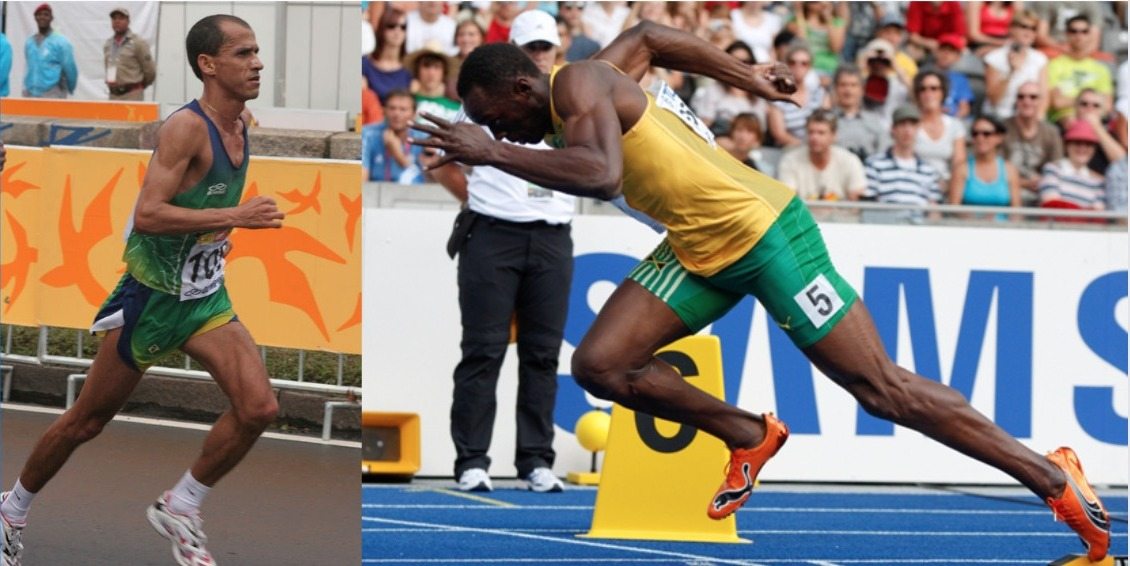
\includegraphics[width=\linewidth]{Figuras/Artigo4/corredores.jpeg}
    \caption{A esquerda, o maratonista Vanderlei Cordeiro de Lima. A direita o velocista Usain Bolt. [Fonte:  \href{https://museuescola.ibb.unesp.br/subtopico.php?id=2&pag=2&num=3&sub=25}{Museu Escola}]}
    \label{corredores2}
\end{figure}

Note que os músculos do corredor de $100$ m rasos são bem maiores e mais desenvolvidos do que os músculos do maratonista. Isso está diretamente ligado à potência que o músculo pode desenvolver. Dentro da fisiologia de um músculo, quando queremos algo com maior eficiência em tempos curtos, ou seja, movimentos explosivos, a melhor estrutura é alcançada com fibras que quando fortalecidas ficam mais grossas, aumentando o volume do músculo de maneira significativa. Enquanto isso, quando se tem como objetivo realizar movimentos de intensidade moderada por um longo período de tempo, a estratégia é que o músculo seja resistente e capaz de aplicar um força por um tempo bem maior. Nesse caso, a estrutura muscular que alcança esse resultado é aquela com fibras que mesmo fortes não variam muito de tamanho, como podendo ser observado na perna do corredor de maratonas.

Toda a análise realizada aqui foi uma grande aproximação para que eu tentasse demonstrar a você, caro leitor, essa conexão entre Física e Esportes. Por meio da aplicação de conceitos básicos relacionados à Física, podemos desenvolver nosso entendimento sobre as modalidades esportivas e assim aumentar muito mais a nossa percepção sobre movimentos e jogadas que muitas vezes parecem impossíveis. Não é necessário que tudo seja regrado fixamente pela matemática, afinal, como já foi dito, somos capazes de realizar cálculos ``de cabeça'' de uma maneira muito dinâmica através de aproximações e experiências. É exatamente isso que um atleta faz ao lançar uma bola de basquete, ele calcula a força e o ângulo necessário para que ao efetuar a jogada, a bola caia exatamente no centro do aro que configura a cesta e assim marca o ponto para o seu time. Usando esses métodos, somos capazes de entender não só um pouco mais de Física e de Esportes, como também de vários outros aspectos do mundo que nos cerca, basta um pouco de curiosidade e interesse, assim como é com esse amor mundial pelos esportes.

\authorinfo{Vítor Hugo Ribeiro}{http://lattes.cnpq.br/3783591692429936}


\end{multicols}
    \protect% Título e referências na mesma página
\mytitle{Referências}% Título da seção de referências[]
\vspace{.5cm}
% Use \ref{ref1:artigo1} para citar uma referência no texto ou \refdois{ref1:artigo1}{ref2:artigo1} e \reftres{ref1:artigo1}{ref2:artigo1}{ref3:artigo1} para citar duas ou três referências.. para mais de três crie um ambiente parecido com o que define esses novos comandos em Structure.tex

\artigoum 
% Ambiente de referências, não se esqueça de alterar a entrada em \label toda vez que for adicionar uma nova referência
\begin{enumerate}
    \item \label{ref1:artigo1} GUTH, Alan H. \textit{The Inflationary Universe: The Quest For a New Theory of Cosmic Origins}. [S.l.]: Helix Books, 1997. v. 33-57, Chapter 3: The birth of modern cosmology, p. 3357.
    \item \label{ref2:artigo1} Canal D-Dimensões. \textit{Big Bang: História e Evidências}. Disponível  \href{https://www.youtube.com/watch?v=ZaVhQJg5j0c&t}{{\tt aqui}}. Acessado em 28/11/2021, às 21:32.
    \item \label{ref3:artigo1} RYDEN, Barbara. \textit{Introduction to cosmology}. [S.l.]: Cambridge University Press, 2017. 5.
    \item \label{ref4:artigo1} PETER, Patrick; UZAN, Jean-Philippe. \textit{Primordial cosmology}. [S.l.]: Oxford University Press, 2013.
\end{enumerate}

%\artigodois
%\begin{enumerate}
%    \item \label{ref1:artigo2}  Entendendo Caravaggio: luz, sombra e uma técnica revolucionária. Disponível clicando \href{https://www.youtube.com/watch?v=cSdF_3touuk}{aqui}.
%    \item \label{ref2:artigo2} Caravaggio, o Gênio Amaldiçoado - Aula Gratuita. Disponível clicando \href{https://www.youtube.com/watch?v=peR3MzJnxOQ}{aqui}. 
%    \item \label{ref3:artigo2} O Mestre dos Pincéis e da Espada. Disponível clicando \href{https://www.youtube.com/watch?v=O1B-jmmeYdI}{aqui}.
%    \item \label{ref4:artigo2} A Inspiração de São Mateus. Disponível clicando \href{https://pt.wikipedia.org/wiki/A_Inspira\%C3\%A7\%C3\%A3o_de_S\%C3\%A3o_Mateus}{aqui}.
%    \item \label{ref5:artigo2} Caravaggio. Disponível clicando \href{https://pt.wikipedia.org/wiki/Caravaggio}{aqui}.
%    \item \label{ref6:artigo2} MICHELANGELO CARAVAGGIO (História da Arte - \#09). Disponível clicando \href{https://www.youtube.com/watch?v=xLtIUxQTxtQ}{aqui}.
%    \item \label{ref7:artigo2} GOMBRICH, E. H. A história da arte. Rio de Janeiro: LTC Livros Téc- nicos e Científicos, 1995.
%    \item \label{ref8:artigo2} GE Física. ed 2 - 2014. (ISBN 789-3614-09105 1) pp.84-85. A Geometria da Luz.
%    \item \label{ref9:artigo2} ``Luz - Comportamento e princípios'' em Só Física. Virtuous Tecnologia da Informação, 2008-2022. Disponível clicando \href{http://www.sofisica.com.br/conteudos/Otica/Fundamentos/luz.php}{aqui}.
%    \item \label{ref10:artigo2} Oxford Languages and Google. Disponível clicando \href{https://languages.oup.com/google-dictionary-pt/}{aqui}. 
%\end{enumerate}

\artigotres
\begin{enumerate}
    \item \label{ref1:artigo3} O que é radiação? Noções básicas de proteção radiológica. Sapra landauer, [SD]. Disponível clicando \href{https://www.sapralandauer.com.br/protecao-radiologica-saiba-sobre-os-principais-aspectos-normas-e-tecnologias-empregadas/o-que-e-radiacao-nocoes-basicas-de-protecao-radiologica/}{aqui.} Acesso em: 6 jun. 2022.
    \item \label{ref2:artigo3} SILVA, J.M. et al. Radiação. \textbf{Mundo educação}, [SD]. Disponível clicando \href{https://mundoeducacao.uol.com.br/quimica/radiacoes.htm}{aqui.} Acesso em: 6 jun. 2022.
    \item \label{ref3:artigo3} RIBEIRO, Sanderson Carlos. text. Wilhelm Conrad Röntgen (1845-1923). Sl, 2 mar. 2018. Disponível clicando \href{https://www3.unicentro.br/petfisica/2018/03/02/wilhelm-conrad-rontgen-1845-1923/}{aqui.} Acesso em: 6 jun. 2022.
    \item \label{ref4:artigo3} SANTOS, Gabriel Grube. text. Antoine Henri Becquerel (1852-1908). Sl, 22 jun. 2017. Disponível clicando \href{https://www3.unicentro.br/petfisica/2017/06/22/antoine-henri-becquerel-1852-1908/}{aqui.} Acesso em: 6 jun. 2022.
    \item \label{ref5:artigo3} DIAS, Diogo Lopes. ``Marie Curie''. \textbf{Brasil Escola} [SD]. Disponível clicando \href{https://www.astropt.org/2014/04/09/movimento-browniano/}{aqui.} Acesso em: 6 jun. 2022.
    \item \label{ref6:artigo3} Radiação. [SL], [SD]. Disponível clicando \href{http://www.fiocruz.br/biosseguranca/Bis/lab_virtual/radiacao.html}{aqui.} Acesso em: 6 jun. 2022.
    \item \label{ref7:artigo3} ABUALROOS, Nadin Jamal et al. Conventional and new lead-free radiation shielding materials for radiation protection in nuclear medicine: A review. \textbf{Radiation Physics and Chemistry}, [s.l.], ano 2019, v. 165, n. 108439, 2019. DOI doi.org/10.1016/j.radphyschem.2019.108439. Disponível clicando \href{https://www.sciencedirect.com/science/article/abs/pii/S0969806X19305699}{aqui.} Acesso em: 6 jun. 2022.
    \item \label{ref8:artigo3} SAYYED, M.I. et al. Effect of ZnO on radiation shielding competence of TeO2-ZnO-Fe2O3 glass system. \textbf{Optik}, [s. l.], ano 2022, v. 249, n. 168270, 2022. DOI doi.org/10.1016/j.ijleo.2021.168270. Disponível clicando \href{https://www.sciencedirect.com/science/article/abs/pii/S0030402621017903?via\%3Dihub}{aqui.} Acesso em: 6 jun. 2022.
    \item \label{ref9:artigo3} Radiação. [SD]. Disponível clicando \href{https://www.fisica.net/aplicada/biofisica/radiacao.php}{aqui.} Acesso em: 6 jun. 2022.
\end{enumerate}

\artigoquatro
\begin{enumerate}
    \item \label{ref1:artigo4} VÍRGULA. Quantas calorias os atletas olímpicos perderam durante as provas?. Disponível cliclando \href{https://www.virgula.com.br/saude/quantas-calorias-os-atletas-olimpicos-perderam-durante-as-provas-nos-te-contamos/}{aqui.}
    \item \label{ref2:artigo4} \textit{NutriRunners}. Velocista x Maratonista - porque corpos tão diferentes?. Disponível cliando \href{https://www.youtube.com/watch?v=kQ7VOb-yzgg}{aqui.}
\end{enumerate}

\begin{center}
    \textcolor{base}{\MakeUppercase{Figuras da Capa e Sumário}}
\end{center}

Figuras da capa: \href{https://www.britannica.com/science/cosmic-microwave-background}{CMB} e \href{https://www.canva.com/}{Fundo da capa};

Figura da contra-capa: \href{https://www.eso.org/public/images/eso1205a/}{Nebulosa Helix - EOS};

Figuras do sumário:

\begin{itemize}
    \item[i)] \href{https://www.sciencephoto.com/media/334059/view}{História do Universo};
    \item[ii)] \href{https://www.wikiart.org/pt/caravaggio}{À Luz de Caravaggio};
    \item[iii)] \href{https://radioprotecaonapratica.com.br/voce-sabe-o-que-e-radiacao/}{Tipos de Radiação};
    \item[iv)] \href{https://www2.ifsc.usp.br/portal-ifsc/a-fisica-no-esporte/}{Física dos Esportes};
\end{itemize}





    \protect\newpage
\thispagestyle{empty}
% Adicione o TikZ para desenhar a linha vertical
\begin{tikzpicture}[remember picture, overlay]
    \draw[line width=3.4cm, base] ($(current page.north east) - (0,0)$) -- ($(current page.south east) - (0,0)$);
\end{tikzpicture}

\vspace{-1cm} % Espaço vertical para mover a figura para cima e caber na página (ajuste de acordo com o modelo, mantendo na página com uma linha vertical de cor referente a base)
\noindent % Evita indentação
\begin{minipage}{7.7cm}% Define a largura da minipage igual à largura da figura
\protect\vspace{16.5cm}% Ajuste fino para mover nota verticalmente
  \large{{\clearsansbold Nota do autor:} \clearsansthin Os outros personagens que aparecem nesta tirinha são o Prof. Cloro e Estrôncio, que também estão em outras tirinhas de minha criação. Aqui, apresenta-se a origem do Sir Apple em uma coletânea de tirinhas especiais. A história continua...}
\end{minipage}
\hspace*{\fill} % Empurra a figura para a direita (caso não use a nota do autor então evite pular linha entre o \end{tikzpicture} da linha vertical e \hspace*{\fill} )
% Tirinha 
\begin{minipage}{9cm} % Define a largura da minipage igual à largura da figura
    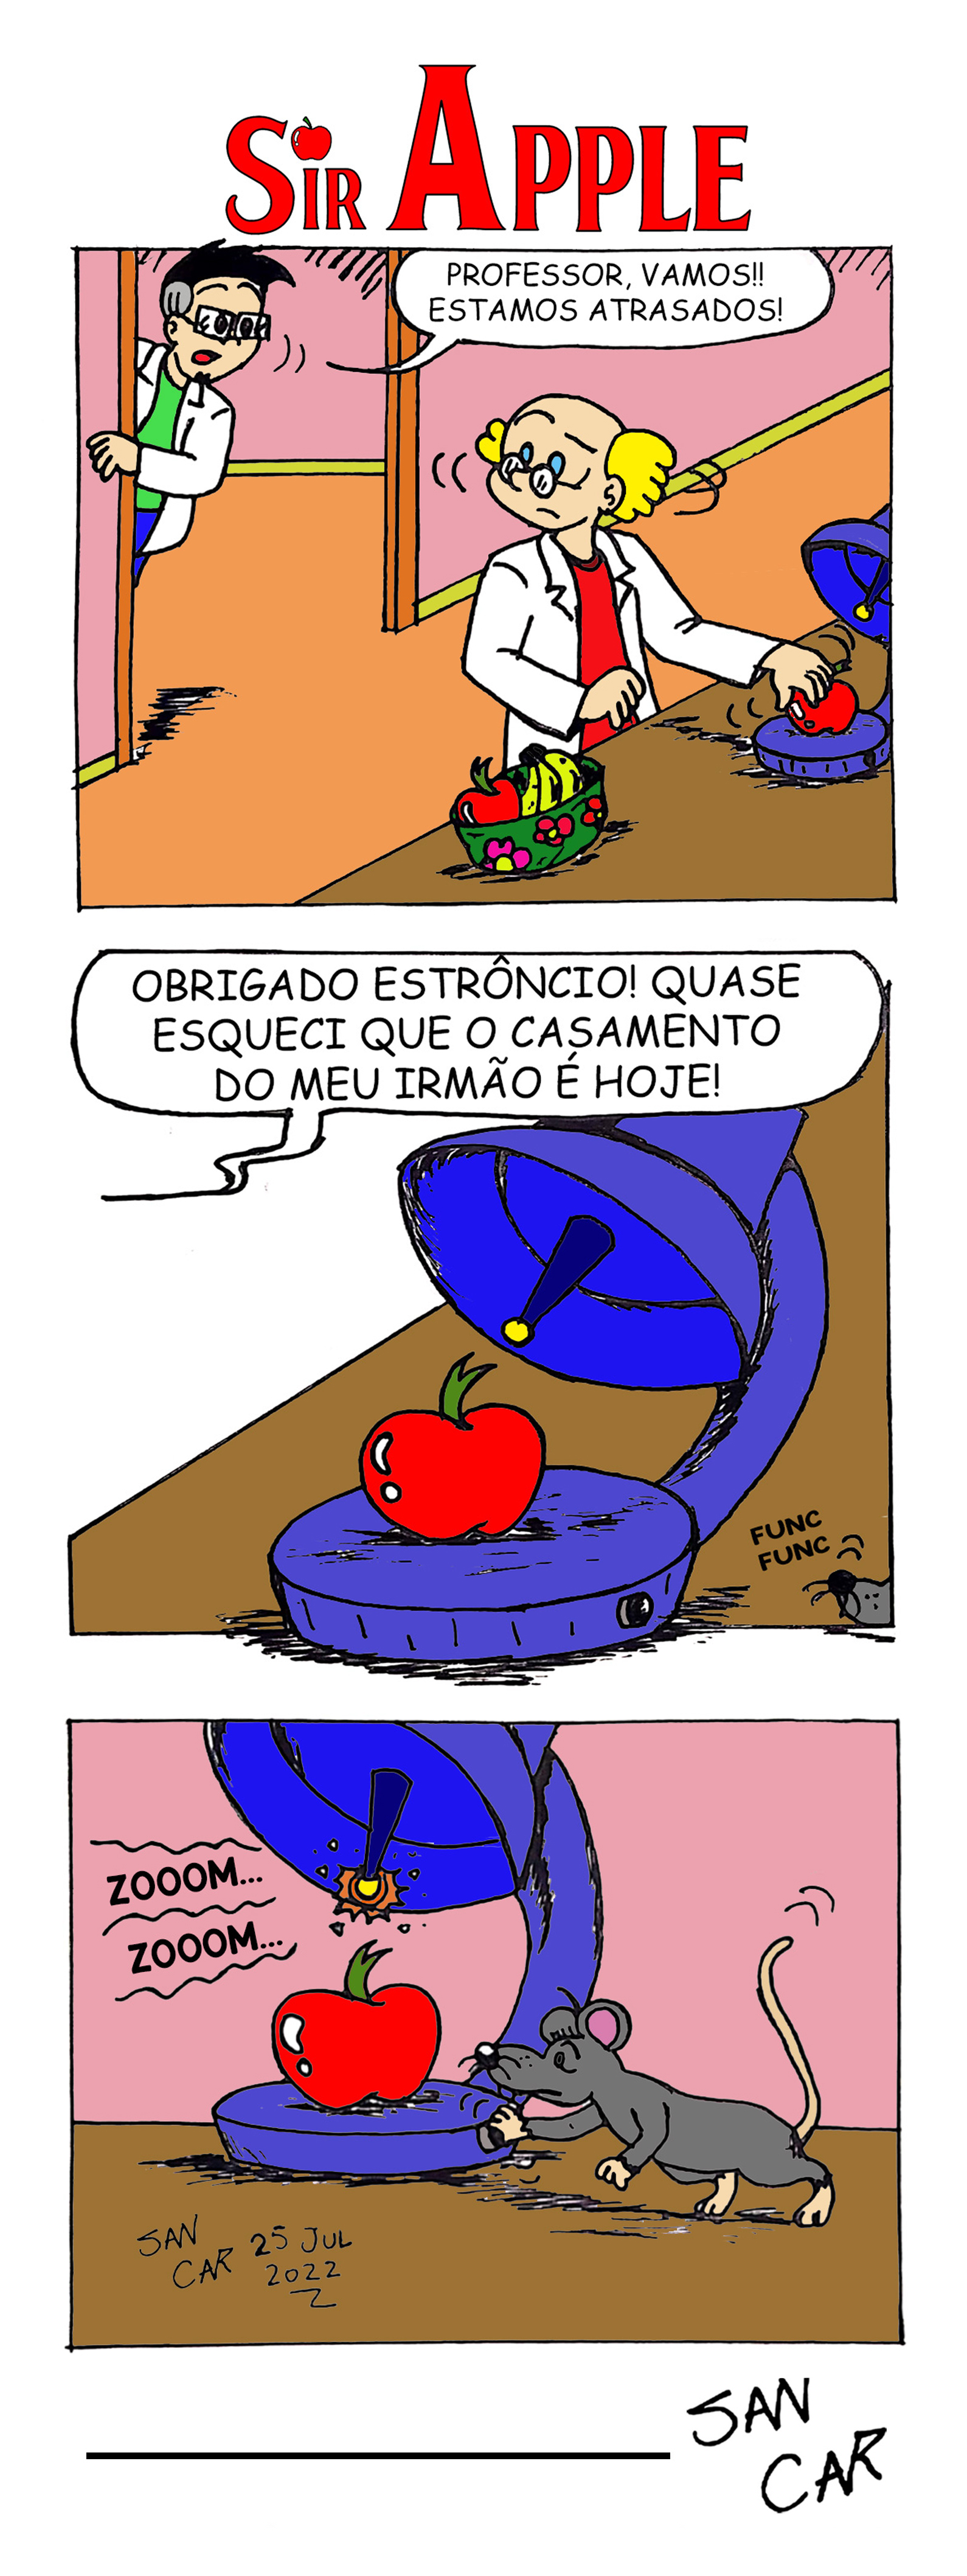
\includegraphics[width=\textwidth]{Tirinha/Tirinha_Fig/Tirinha_Sir_Apple.jpg}
\end{minipage}











    \protect\newpage
\thispagestyle{empty}
% Linhas verticais Contra Capa
\begin{tikzpicture}[remember picture, overlay]
    \draw[line width=3.1cm, base] ($(current page.north east) - (0,0)$) -- ($(current page.south east) - (0,0)$);
    \draw[line width=1.05cm, base] ($(current page.north east) - (2.25,0)$) -- ($(current page.south east) - (2.25,0)$);
    \draw[line width=22.6cm, base] ($(current page.north east) - (14.25,0)$) -- ($(current page.south east) - (14.25,0)$);
\end{tikzpicture}

% Texto
\begin{tikzpicture}[remember picture, overlay]
  % Adiciona texto
  \node at (current page.north west) [anchor=north west, xshift=2cm, yshift=-3cm] {\begin{minipage}[t]{8cm} % Define a largura da minipage igual à largura da figura
  \setlength{\baselineskip}{1.5\baselineskip}
    {\clearsansthin\myfontsizeTemaCapaVerticalECC O Newston Jornal surgiu como uma iniciativa estudantil envolvendo alunos dos cursos de Física, Letras e Arquitetura e Urbanismo da Universidade Estadual de Maringá (UEM) em 2018, e foi oficializado como projeto de extensão vinculado oficialmente à universidade em março de 2021.} \end{minipage}
  };
   \node at (current page.north west) [anchor=north west, xshift=2cm, yshift=-10.5cm] {\begin{minipage}[t]{8cm} % Define a largura da minipage igual à largura da figura
  \setlength{\baselineskip}{1.5\baselineskip}
    {\clearsansthin\myfontsizeTemaCapaVerticalECC Desde o início, a finalidade do projeto consiste em produzir material para divulgação científica e cultural que atenda à comunidade externa e interna da universidade, visando sempre a integração de diversas áreas do conhecimento.} \end{minipage}
  };
\end{tikzpicture}

% Logo do Newston e da UEM
\begin{tikzpicture}[remember picture, overlay]
  % Adiciona a logo maçã branco
  \node at (current page.north west) [anchor=north west, xshift=2cm, yshift=-25.7cm] {
    
\includegraphics[width=1.5cm]{Sumario/Figs_Sumario/Logo_Maca_Branco.png}
  };
    % Adiciona o texto Newston
  \node at (current page.north west) [anchor=north west, xshift=3.8cm, yshift=-26cm] {
    {\norwester\myfontsizeNewstonSumarioECC NEWSTON}
  };
   % Adiciona o texto Jornal
  \node at (current page.north west) [anchor=north west, xshift=3.85cm, yshift=-27cm] {
    {\bebasneue\myfontsizeJornalSumarioECC \textls[590]{JORNAL}}
  };
  % Adiciona a logo da UEM Branco
  \node at (current page.north west) [anchor=north west, xshift=12.5cm, yshift=-25.7cm] {
    
\includegraphics[width=0.22\textwidth]{Figuras_Capa_ContraCapa/UEM_Logo_Modelo_Branco.png}
  };
\end{tikzpicture}


    
\end{document}

% Comandos LaTex desenvolvidos por Sanderson Carlos Ribeiro (e-mail: San.Car.Oficial@gmail.com) com o auxílio do ChatGPT. Design da Edição por Vítor Hugo Ribeiro (e-mail: vitorhibeiro@gmail.com).